% Options for packages loaded elsewhere
% Options for packages loaded elsewhere
\PassOptionsToPackage{unicode}{hyperref}
\PassOptionsToPackage{hyphens}{url}
\PassOptionsToPackage{dvipsnames,svgnames,x11names}{xcolor}
%
\documentclass[
]{scrartcl}
\usepackage{xcolor}
\usepackage[left=2.5cm,right=2.5cm,top=3cm,bottom=3cm]{geometry}
\usepackage{amsmath,amssymb}
\setcounter{secnumdepth}{5}
\usepackage{iftex}
\ifPDFTeX
  \usepackage[T1]{fontenc}
  \usepackage[utf8]{inputenc}
  \usepackage{textcomp} % provide euro and other symbols
\else % if luatex or xetex
  \usepackage{unicode-math} % this also loads fontspec
  \defaultfontfeatures{Scale=MatchLowercase}
  \defaultfontfeatures[\rmfamily]{Ligatures=TeX,Scale=1}
\fi
\usepackage{lmodern}
\ifPDFTeX\else
  % xetex/luatex font selection
\fi
% Use upquote if available, for straight quotes in verbatim environments
\IfFileExists{upquote.sty}{\usepackage{upquote}}{}
\IfFileExists{microtype.sty}{% use microtype if available
  \usepackage[]{microtype}
  \UseMicrotypeSet[protrusion]{basicmath} % disable protrusion for tt fonts
}{}
\makeatletter
\@ifundefined{KOMAClassName}{% if non-KOMA class
  \IfFileExists{parskip.sty}{%
    \usepackage{parskip}
  }{% else
    \setlength{\parindent}{0pt}
    \setlength{\parskip}{6pt plus 2pt minus 1pt}}
}{% if KOMA class
  \KOMAoptions{parskip=half}}
\makeatother
% Make \paragraph and \subparagraph free-standing
\makeatletter
\ifx\paragraph\undefined\else
  \let\oldparagraph\paragraph
  \renewcommand{\paragraph}{
    \@ifstar
      \xxxParagraphStar
      \xxxParagraphNoStar
  }
  \newcommand{\xxxParagraphStar}[1]{\oldparagraph*{#1}\mbox{}}
  \newcommand{\xxxParagraphNoStar}[1]{\oldparagraph{#1}\mbox{}}
\fi
\ifx\subparagraph\undefined\else
  \let\oldsubparagraph\subparagraph
  \renewcommand{\subparagraph}{
    \@ifstar
      \xxxSubParagraphStar
      \xxxSubParagraphNoStar
  }
  \newcommand{\xxxSubParagraphStar}[1]{\oldsubparagraph*{#1}\mbox{}}
  \newcommand{\xxxSubParagraphNoStar}[1]{\oldsubparagraph{#1}\mbox{}}
\fi
\makeatother


\usepackage{longtable,booktabs,array}
\usepackage{calc} % for calculating minipage widths
% Correct order of tables after \paragraph or \subparagraph
\usepackage{etoolbox}
\makeatletter
\patchcmd\longtable{\par}{\if@noskipsec\mbox{}\fi\par}{}{}
\makeatother
% Allow footnotes in longtable head/foot
\IfFileExists{footnotehyper.sty}{\usepackage{footnotehyper}}{\usepackage{footnote}}
\makesavenoteenv{longtable}
\usepackage{graphicx}
\makeatletter
\newsavebox\pandoc@box
\newcommand*\pandocbounded[1]{% scales image to fit in text height/width
  \sbox\pandoc@box{#1}%
  \Gscale@div\@tempa{\textheight}{\dimexpr\ht\pandoc@box+\dp\pandoc@box\relax}%
  \Gscale@div\@tempb{\linewidth}{\wd\pandoc@box}%
  \ifdim\@tempb\p@<\@tempa\p@\let\@tempa\@tempb\fi% select the smaller of both
  \ifdim\@tempa\p@<\p@\scalebox{\@tempa}{\usebox\pandoc@box}%
  \else\usebox{\pandoc@box}%
  \fi%
}
% Set default figure placement to htbp
\def\fps@figure{htbp}
\makeatother


% definitions for citeproc citations
\NewDocumentCommand\citeproctext{}{}
\NewDocumentCommand\citeproc{mm}{%
  \begingroup\def\citeproctext{#2}\cite{#1}\endgroup}
\makeatletter
 % allow citations to break across lines
 \let\@cite@ofmt\@firstofone
 % avoid brackets around text for \cite:
 \def\@biblabel#1{}
 \def\@cite#1#2{{#1\if@tempswa , #2\fi}}
\makeatother
\newlength{\cslhangindent}
\setlength{\cslhangindent}{1.5em}
\newlength{\csllabelwidth}
\setlength{\csllabelwidth}{3em}
\newenvironment{CSLReferences}[2] % #1 hanging-indent, #2 entry-spacing
 {\begin{list}{}{%
  \setlength{\itemindent}{0pt}
  \setlength{\leftmargin}{0pt}
  \setlength{\parsep}{0pt}
  % turn on hanging indent if param 1 is 1
  \ifodd #1
   \setlength{\leftmargin}{\cslhangindent}
   \setlength{\itemindent}{-1\cslhangindent}
  \fi
  % set entry spacing
  \setlength{\itemsep}{#2\baselineskip}}}
 {\end{list}}
\usepackage{calc}
\newcommand{\CSLBlock}[1]{\hfill\break\parbox[t]{\linewidth}{\strut\ignorespaces#1\strut}}
\newcommand{\CSLLeftMargin}[1]{\parbox[t]{\csllabelwidth}{\strut#1\strut}}
\newcommand{\CSLRightInline}[1]{\parbox[t]{\linewidth - \csllabelwidth}{\strut#1\strut}}
\newcommand{\CSLIndent}[1]{\hspace{\cslhangindent}#1}



\setlength{\emergencystretch}{3em} % prevent overfull lines

\providecommand{\tightlist}{%
  \setlength{\itemsep}{0pt}\setlength{\parskip}{0pt}}



 


\usepackage[noblocks]{authblk}
\renewcommand*{\Authsep}{, }
\renewcommand*{\Authand}{, }
\renewcommand*{\Authands}{, }
\renewcommand\Affilfont{\small}
\usepackage{lineno}
\usepackage{scrlayer-scrpage}
\rohead{IOTC-2025-WPTT27-23}
\usepackage{lscape}
\newcommand{\blandscape}{\begin{landscape}}
\newcommand{\elandscape}{\end{landscape}}
\makeatletter
\@ifpackageloaded{caption}{}{\usepackage{caption}}
\AtBeginDocument{%
\ifdefined\contentsname
  \renewcommand*\contentsname{Table of contents}
\else
  \newcommand\contentsname{Table of contents}
\fi
\ifdefined\listfigurename
  \renewcommand*\listfigurename{List of Figures}
\else
  \newcommand\listfigurename{List of Figures}
\fi
\ifdefined\listtablename
  \renewcommand*\listtablename{List of Tables}
\else
  \newcommand\listtablename{List of Tables}
\fi
\ifdefined\figurename
  \renewcommand*\figurename{Figure}
\else
  \newcommand\figurename{Figure}
\fi
\ifdefined\tablename
  \renewcommand*\tablename{Table}
\else
  \newcommand\tablename{Table}
\fi
}
\@ifpackageloaded{float}{}{\usepackage{float}}
\floatstyle{ruled}
\@ifundefined{c@chapter}{\newfloat{codelisting}{h}{lop}}{\newfloat{codelisting}{h}{lop}[chapter]}
\floatname{codelisting}{Listing}
\newcommand*\listoflistings{\listof{codelisting}{List of Listings}}
\makeatother
\makeatletter
\makeatother
\makeatletter
\@ifpackageloaded{caption}{}{\usepackage{caption}}
\@ifpackageloaded{subcaption}{}{\usepackage{subcaption}}
\makeatother
\usepackage{bookmark}
\IfFileExists{xurl.sty}{\usepackage{xurl}}{} % add URL line breaks if available
\urlstyle{same}
\hypersetup{
  pdftitle={Advances in the use of state-space assessment models for tuna stocks: application to the Indian Ocean bigeye tuna},
  colorlinks=true,
  linkcolor={blue},
  filecolor={Maroon},
  citecolor={Blue},
  urlcolor={Blue},
  pdfcreator={LaTeX via pandoc}}


\title{Advances in the use of state-space assessment models for tuna
stocks: application to the Indian Ocean bigeye tuna}


\author[1]{Giancarlo M. Correa}
\author[2]{Genevieve Phillips}
\author[1]{Gorka Merino}
\author[1]{Agurtzane Urtizberea}
\author[3]{Yang Wang}

\affil[1]{AZTI, Marine Research, Basque Research and Technology Alliance
(BRTA), Txatxarramendi ugartea z/g, 48395 Sukarrieta (Bizkaia), Spain}
\affil[2]{Indian Ocean Tuna Commission, Mahe, Seychelles}
\affil[3]{College of Marine Living Resource Sciences and Management,
Shanghai Ocean University, Shanghai, China}


\date{}
\begin{document}
\maketitle


\textbf{Abstract}

The use of the state-space approach in fish stock assessments has
received more attention in recent years and is considered as an
essential feature for the next-generation stock assessment platforms.
However, age-structure state-space asssessment models (SSAMs) are still
uncommon for stocks with scarce age information, like tunas. In this
study, we aimed to apply an age-structured SSAMs (the Woods Hole
Assessment Model - WHAM) to the Indian Ocean bigeye tuna using data
inputs that are common for tuna stocks: aggregated catch, indices of
abundance, and marginal length compositions. Our models suggest that the
SSB has decreased from values around 1.3 million mt in 1979 to values
around 400 thousand mt in 2024. Also, the most likely stock status is
not overfished and not subject to overfishing in 2024, although there is
a high probability (\(\sim 0.45\)) of being subject to overfishing for
most models. We also provided some diagnostics (e.g., retrospective
analysis, likelihood profile, jitter analysis) for the implemented
models, and ran some model projections to show the capabilities of WHAM.
We hope that this study may increase the visibility of age-structured
SSAMs and their application to other tuna stocks as an alternative
platform.

\emph{Keywords}

bigeye tuna, state-space models, stock assessment models, Indian Ocean,
Woods Hole Assessment Model

\newpage

\section{Introduction}\label{introduction}

Age-structured population dynamics models were initially limited to the
use of age-specific data to estimate abundance-at-age and fishing
mortality-at-age. Since the late 1990s, age-structured assessment
platforms have been developed to include size-specific data and model
the age-size transition internally
(\citeproc{ref-fournierMULTIFANCLLengthbasedAgestructured1998}{Fournier
et al., 1998}; \citeproc{ref-methotStockSynthesisBiological2013}{Methot
and Wetzel, 2013}), expanding their use for stocks with scarce age
information like tunas. Most of these platforms were written in AD Model
Builder (ADMB), which allowed for the efficient and accurate estimation
of a large number of parameters
(\citeproc{ref-fournierADModelBuilder2012}{Fournier et al., 2012}).
During the last decade, age-structured state-space assessment models
(SSAMs) have rapidly become popular due to the development of Template
Model Builder (TMB) software, which leverages the Laplace approximation
to efficiently integrate out random effects
(\citeproc{ref-kristensenTMBAutomaticDifferentiation2016}{Kristensen et
al., 2016}). State-space models are a type of hierarchical model with
two levels: 1) unobserved states or processes that represent the true
state of nature that may vary over time, and 2) observations with
associated errors of the state of nature
(\citeproc{ref-auger-metheGuideStateSpace2021}{Auger-Méthé et al.,
2021}). The key strength of models written in TMB is their ability to
estimate process error variation objectively by treating them as random
effects, which is considered an essential feature in next-generation
stock assessment platforms
(\citeproc{ref-puntEssentialFeaturesNextgeneration2020}{Punt et al.,
2020}).

The Stock Synthesis (SS3) platform
(\citeproc{ref-methotStockSynthesisBiological2013}{Methot and Wetzel,
2013}) is written in ADMB and has become very popular to implement
assessment models for tuna stocks worldwide, principally including
catch, indices of abundance, marginal size compositions and, in some
cases, tagging and conditional age-at-length data. Traditionally,
estimating process error variation in models written in ADMB like SS3 is
done using the ``penalized maximum likelihood'' approach, which
estimates penalized deviations
\(\epsilon_y \sim N(0,\sigma_\epsilon^2)\) from the mean parameter while
subjectively fixing or iteratively tuning the penalty term
\(\sigma_\epsilon^2\) (\citeproc{ref-methotAdjustingBiasDue2011}{Methot
and Taylor, 2011}), or approximating it
(\citeproc{ref-thorsonRandomEffectEstimation2015}{Thorson et al.,
2015}).

The State-space Assessment Model -SAM-
(\citeproc{ref-bergAccountingCorrelatedObservations2016}{Berg and
Nielsen, 2016};
\citeproc{ref-nielsenEstimationTimevaryingSelectivity2014}{Nielsen and
Berg, 2014}) and the Woods Hole Assessment Model -WHAM-
(\citeproc{ref-stockWoodsHoleAssessment2021}{Stock and Miller, 2021})
are two popular age-structured SSAM platforms written in TMB that can
model recruitment, age-based selectivity, natural and fishing mortality
or survival, and environmental variables using random effects
(\citeproc{ref-millerTemporalEnvironmentalVariation2018}{Miller et al.,
2018}; \citeproc{ref-millerEvaluatingEvidenceAlternative2018}{Miller and
Hyun, 2018}; \citeproc{ref-stockWoodsHoleAssessment2021}{Stock and
Miller, 2021}). SAM and WHAM are mostly applied to stocks on the east
coast of North America and ICES management zones
(\citeproc{ref-icesHaddockMelanogrammusAeglefinus2024}{ICES, 2024};
\citeproc{ref-nefscButterfishResearchTrack2024}{NEFSC, 2024}; e.g.,
\citeproc{ref-nefscReportBlackSea2023}{NEFSC, 2023}), where plenty of
age information is available.

The use of age-structured SSAM for tuna stocks has been limited,
probably due to the scarce age information for these stocks and the
absence of state-space assessment platforms able to include
size-specific data or model size-based processes. Mhamed et al.
(\citeproc{ref-mhamedEasternBluefinTuna2017}{2017}) applied SAM to
implement a stock assessment model for eastern Atlantic bluefin tuna
(\emph{Thunnus thynnus}), converting marginal size compositions and
aggregated catch and indices of abundance to catch-at-age and
index-at-age data. Correa et al.
(\citeproc{ref-correaModellingTimevaryingGrowth2023}{2023}) extended
WHAM (\emph{growth-WHAM} hereafter) to model length-based processes such
as selectivity and growth and to allow the use of length compositions or
conditional age-at-length (CAAL) as data inputs. Likewise, other size-
or age-structured SSAMs have been developed to model these processes as
length-based rather than age-based
(\citeproc{ref-hillaryIntegratedStockAssessment2021}{Hillary and Day,
2021}; \citeproc{ref-zhangAgeLengthStructured2022}{Zhang and Cadigan,
2022}). These developments could expand the use of age-structured SSAMs
to fish stocks with scarce age information like tunas.

In this study, we implemented a stock assessment model for Indian Ocean
(IO) bigeye tuna in WHAM. The source of data to derive the model data
inputs (catch, indices of abundance, marginal size compositions) was the
same as that used in the SS3 IO bigeye assessment model presented in the
Working Party of Tropical Tunas 27th (WPTT27). The model configurations
considered uncertainty in key fishery processes (e.g., selectivity) and
data inputs. We also show examples of WHAM capabilities to estimate
stock status and conduct model diagnostics and projections. The main
goal of this study is to introduce WHAM to the tuna RFMOs, and increase
the use of age-structure SSAMs for tuna stocks since they may become
more popular in future years.

\section{Methods}\label{methods}

\subsection{Model inputs}\label{model-inputs}

Catch (1979-2024) and size (1979-2024) information was provided by the
IOTC Secretariat in a comma-separated values (CSV) format. Two indices
of abundance were also available: joint longline and purse seine fishing
on associated schools. These indices can also be found online at
\url{https://iotc.org/documents/standardised-cpue-index-bigeye-tuna}.

\subsection{Definition of fisheries}\label{definition-of-fisheries}

Our assessment adopted the equivalent fisheries definitions used in the
previous SS3 stock assessments. Seven \emph{fishery groups} were defined
based on fleet, gear, purse seine set type, and type of vessel in the
case of the longline fleet (Table~\ref{tbl-fishery-codes}), representing
relatively homogeneous fishing units with similar selectivity and
catchability characteristics that do not vary greatly over time.

A brief description of each \emph{fishery group} is provided below.

\begin{itemize}
\item
  \emph{Freezing longline fisheries (LL)}, or all those using drifting
  longlines for which one or more of the following three conditions
  apply: (i) the vessel hull is made up of steel; (ii) the vessel length
  overall of 30 m or greater; (iii) the majority of the catches of
  target species are preserved frozen or deep-frozen.
\item
  \emph{Fresh-tuna longline fisheries (LF)}, or all those using drifting
  longlines and made of vessels (i) having fibreglass, fibre-reinforced
  plastic, or wooden hull; (ii) having length overall less than 30 m;
  (iii) preserving the catches of target species fresh or in
  refrigerated seawater.
\item
  The purse-seine catch and effort data were apportioned into two
  separate fisheries: catches from sets on associated schools of tuna
  (log and drifting FAD sets; \emph{PSLS}) and sets on unassociated
  schools (free schools; \emph{PSFS}).
\item
  Baitboat fishery (\emph{BB}), which included the pole-and-line
  (essentially the Maldives fishery) and small seine fisheries (catching
  small fish).
\item
  Line fishery (\emph{LINE}), representing a mixture of gears using
  handlines, and small longlines (including the gillnet and longline
  combination fishery of Sri Lanka).
\item
  A miscellaneous ``Other'' fishery (\emph{OTHER}) was defined,
  comprising catches from artisanal fisheries other than those specified
  above (e.g.~gillnet, trolling and a range of small gears).
\end{itemize}

These fishery groups were used as the model fleets in WHAM.

\subsection{Aggregated catch}\label{aggregated-catch}

The catch dataset was composed of information about time (year and
month), CPCs, gear type, type of association of the fish school, grid
code at a \(5^\circ\times 5^\circ\) resolution, and catch in weight
(metric tons) and numbers. The grid code contained information on the
grid resolution, quadrant, and longitude and latitude of the corner of
the grid.

To process this dataset and generate the catch inputs for WHAM, we first
identified the fishery groups based on CPC, gear type, and the type of
association of the fish school. Then, catch was summed by year and
fishery group (Figure~\ref{fig-catch}).

\subsection{Size data}\label{sec-size}

The size data was composed of information about time (year and month),
CPC, gear type, type of association of the fish school, grid code,
number of fish sampled per fork length bin (cm), and the score of
reporting quality (RQ). The RQ score is a proxy of the quality (e.g.,
sampling coverage, reporting details) of the size information provided
to the IOTC Secretariat by CPCs
(\citeproc{ref-herreraProposalSystemAssess2010}{Herrera, 2010};
\citeproc{ref-iotcReviewStatisticalData2024}{IOTC, 2024}). The length
bin width was 2 cm and the length bins spanned from 10 to 340 cm. The
size dataset had six main types of grid dimensions, although most of
them were category 5 (\(1\times 1^\circ\)) or 6 (\(5\times 5^\circ\)).
The data were collected from a variety of sampling programs, which are
described in Fu et al.
(\citeproc{ref-fuPreliminaryIndianOcean2022}{2022}).

To process this dataset and generate the size compositions inputs for
WHAM, we first filtered the data to remove inconsistent size samples
using the criterion followed in official 2025 IO bigeye stock
assessment. Then, we identified the fishery groups based on CPC, gear
type, and the type of association of the fish school. Then, we reduced
the number of length bins in the data by summing the number of sampled
fish \(\geq\) 198 cm and assigning it to the 198 cm length bin. The
fishery group was assigned based on the CPC, gear type, and type of
association of the fish school. Then, we converted the length bin width
from 2 to 4 cm. To do so, we summed the number of sampled fish from
pairs of length bins (e.g., 10 and 12 cm were summed and assigned to 10
cm, 14 and 16 cm were summed and assigned to 14 cm, and so on). After
this conversion, we had a total of 48 length bins. Finally, the number
of sampled fish per length bin was summed and the RQ was averaged by
year and fishery group (Figure~\ref{fig-len-1}, Figure~\ref{fig-len-2},
Figure~\ref{fig-len-3}, Figure~\ref{fig-len-4}, Figure~\ref{fig-len-5},
Figure~\ref{fig-len-6}, Figure~\ref{fig-len-7}).

The RQ was used as input sample size in WHAM. Due to lower scores of RQ
represent better quality, we inverted the RQ scores from a minimum of 5
(corresponded to an original RQ of 6) and maximum of 20 (corresponded to
an original RQ of 0). Also, we removed size compositions for for
\emph{LINE}, \emph{OTHER}, \emph{BB} fisheries before 2008 due to
inconsistent samples.

\subsection{Indices}\label{indices}

\subsubsection{Longline (LL) CPUE}\label{sec-llcpue}

Standardised LL CPUE indices (1979-2024) were available from a joint
workshop held by Japan, Korea, and Taiwan
(\citeproc{ref-kitakadoUpdateJointCPUE2025}{Kitakado et al., 2025}). The
indices were derived following the methodology developed for previous
stock assessments and were provided for the four assessment areas used
in the last assessment model
(\citeproc{ref-fuPreliminaryIndianOcean2022}{Fu et al., 2022}) in a
quarterly temporal resolution.

We determined regional scaling factors that incorporated both the size
of the region and the relative catch rate to estimate the relative level
of exploitable longline biomass among regions (method `8' in Hoyle and
Langley (\citeproc{ref-hoyleScalingFactorsMultiregion2020}{2020})).
After scaling the indices by region, we grouped them by summing the
values by quarter. Then, we grouped this index by year by averaging the
LL CPUE quarterly values (Figure~\ref{fig-index}). A coefficient of
variation (CV) of 0.1 was assumed for all years.

\subsubsection{Purse seine (PSLS) CPUE}\label{purse-seine-psls-cpue}

A standardised index of the biomass of bigeye caught by European purse
seiners (Spain and France) from sets on associated tuna schools (1991 --
2023) was developed
(\citeproc{ref-correaStandardizedCatchUnit2025}{Correa et al., 2025})
and provided in a quarterly temporal resolution. Data used to develop
this index mainly come from the western IO and mainly informs on the
biomass of juvenile bigeye. We averaged the quarterly CPUE values by
year to be included in WHAM (Figure~\ref{fig-index}). The CV associated
with each quarterly value was also averaged and then rescaled to a mean
of 0.2 to be used as observation error.

\section{Model parameters}\label{model-parameters}

\subsection{Population dynamics}\label{population-dynamics}

The model configurations were single-area and partitioned the population
into 10 yearly age classes (\(1-10+\)), both sexes combined. The last
age-class (\(10+\)) comprises a \emph{plus group} in which mortality and
other characteristics are assumed to be constant. Age quantities are
partitioned into 48 4-cm length bins ranging from 10 to 198 cm, which
covers the main size range observed for bigeye in the IO. The population
is monitored in the model at yearly time steps, extending through a time
window of 1979--2024. The main population dynamics processes are as
follows.

\subsubsection{Recruitment}\label{recruitment}

Recruitment in WHAM is defined as the appearance of age-1 fish in the
population. Recruitment was assumed to be a function of spawning biomass
via a Beverton and Holt stock-recruitment relationship (SRR) with a
fixed value of steepness (\(h\)). Typically, fisheries data are not very
informative about the steepness parameter of the SRR parameters
(\citeproc{ref-leeCanSteepnessStock2012}{Lee et al., 2012}); hence, the
steepness parameter was fixed at a moderate value (0.80). Deviates from
the SRR curve (\emph{recruitment deviates}) were modelled from 1979 to
2024 as random effects while its standard deviation (\(\sigma_R\)) was
estimated.

\subsubsection{Initial population}\label{initial-population}

The population age structure at the start of the first year (i.e., 1979)
was assumed to be in equilibrium state, estimating the number of fish at
age 1 (\(N1\)) and an initial fishing mortality to derive the abundance
of other age classes.

\subsubsection{Somatic growth and sexual maturity}\label{sec-growth}

The 2022 bigeye stock assessment used growth parameters that replicated
the growth curve derived by Eveson et al.
(\citeproc{ref-evesonUpdatedGrowthEstimates2012}{2012}). In the WPTT(DP)
27, Eveson et al. (\citeproc{ref-evesonUpdatingEstimationAge2025}{2025})
presented growth estimates using otolith information from the GERUNDIO
project and found quite different growth patterns compared to previous
studies. In our WHAM assessment models, we use the Eveson et al.
(\citeproc{ref-evesonUpdatingEstimationAge2025}{2025}) estimates by
modelling a von Bertalanffy growth curve (Figure~\ref{fig-growth}). For
the length-weight relationship, we use the estimates found in Chassot et
al. (\citeproc{ref-chassotLengthweightRelationshipsTropical2016}{2016}).
Regarding sexual maturity, we modelled size-based logistic maturity
using the parameters from the last stock assessment held in 2022.
Parameters related to somatic growth and fixed in our models are shown
in Table~\ref{tbl-par-fix}.

\subsubsection{Natural mortality}\label{natural-mortality}

For the current assessment, we used the \(M_a\) estimates following
Hamel and Cope
(\citeproc{ref-hamelDevelopmentConsiderationsApplication2022}{2022}) and
then rescaled based on Lorenzen
(\citeproc{ref-lorenzenPopulationDynamicsPotential2005}{2005}). This
relationship models high \(M\) for younger fish, which then declines as
fish get older. In WHAM, the reference natural mortality is calculated
from \(M_{ref} = 5.4/A_{max}\), where \(A_{max}\) is the assumed maximum
age in the population equal to 14.7 years based on Eveson et al.
(\citeproc{ref-evesonUpdatingEstimationAge2025}{2025}). \(M_{ref}\) is
the natural mortality that corresponds to the age at the 95\% maturity,
assumed to be 3.75 years based on the maturity and growth curve. Then,
the rescaling of natural mortality at age is performed as a function of
the \(L_\infty\) and \(k\) growth parameters (Figure~\ref{fig-Matage}).

\subsection{Fishery dynamics}\label{fishery-dynamics}

\subsubsection{Fishing mortality}\label{fishing-mortality}

Yearly fishing mortality per fleet was estimated as fixed effect through
the use of fishing deviates.

\subsubsection{Catchability}\label{catchability}

We estimated the catchability parameters for each index (\emph{LL} and
\emph{PSLS}) included in the stock assessment model.

\subsubsection{Selectivity}\label{selectivity}

Selectivity was assumed to be size-based for all fleets in our model.

\begin{itemize}
\item
  Longline (\emph{LL}): parameterised with a logistic function that
  constrains the older age classes to be fully selected (``flat top'').
  Some model configurations also modelled time-variant selectivity with
  two blocks: before and after 2000, with a logistic parametrization
  after 2000 and dome-shaped before 2000. The \emph{LL} CPUE index was
  linked to this selectivity.
\item
  Purse seine on free schools (\emph{PSFS}): modelled using cubic
  splines with five nodes. The nodes were specified to approximate the
  main inflection points of the selectivity function.
\item
  Purse seine on log schools (\emph{PSLS}): modelled using a
  double-normal parametrization. The \emph{PSLS} CPUE index was linked
  to this selectivity.
\item
  Longline fresh tuna (\emph{FL}): parameterised with a logistic
  function that constrains the older age classes to be fully selected
  (``flat top'').
\item
  Line (\emph{LINE}): parameterised with a logistic function.
\item
  Baitboat (\emph{BB}): mirrored the selectivity of the \emph{PSLS}
  fishery.
\item
  Other (\emph{OTHER}): mirrored the selectivity of the \emph{PSFS}
  fishery.
\end{itemize}

\subsection{Likelihood components}\label{likelihood-components}

The total likelihood is composed of a number of components, including
the fit to the catch data, indices of abundance (CPUE), and length
frequency data. There are also contributions to the total likelihood
from the recruitment deviates and priors on the individual model
parameters.

\subsubsection{Catch}\label{catch}

The catch data assumed a lognormal error structure. There is no
objective estimates of the degree in uncertainty in aggregated catch
data, therefore, like in the 2022 assessment, we assumed a value of 0.1
for every observation.

\subsubsection{Indices of abundance}\label{indices-of-abundance}

The CPUE indices assumed a lognormal error structure. The 2022
assessment assumed a CV for every \emph{LL} CPUE observation of 0.1. In
the current assessment, we followed the same approach. For the
\emph{PSLS} index, we used the CV derived from the standardization
method.

\subsubsection{Length frequency}\label{length-frequency}

The length frequency assumed a multinomial error structure. The current
assessment treated the RQ values (see Section~\ref{sec-size}) as the
input sample size.

\subsubsection{Recruitment}\label{recruitment-1}

Derived from the estimation of annual recruitment as random effects.

\subsection{Parameter estimation and
uncertainty}\label{parameter-estimation-and-uncertainty}

The parameters of the model were estimated by minimising the sum of the
negative log-likelihood components associated with each of the data
components plus the negative log of the probability density functions of
recruitment deviates. Models were run with a gradient criterion of
\(10^{-4}\). The Hessian matrix computed at the mode of the posterior
distribution was used to obtain estimates of the covariance matrix,
which was used in combination with the Delta method to compute
approximate confidence intervals for parameters of interest.

The structural uncertainty grid attempts to describe the main sources of
structural and data uncertainty in the assessment. For the current
assessment, we have continued with a factorial grid of model runs which
incorporates the following sources of uncertainties
(Table~\ref{tbl-mod-config}):

\begin{itemize}
\tightlist
\item
  Selectivity of the \emph{LL} fishery: constant over the years or with
  two blocks: before and after 2002.
\item
  Including or excluding the \emph{PSLS} CPUE index.
\end{itemize}

\subsubsection{Diagnostics}\label{diagnostics}

In order to evaluate model misspecification, we applied a series of
diagnostics tools described in Carvalho et al.
(\citeproc{ref-carvalhoCookbookUsingModel2021}{2021}) to the four model
configurations. Regarding convergence, we examined the maximum final
gradient, invertible Hessian, and ran a jittering analysis to evaluate
if models converged to a global solution.

For highly complex population models fitted to large amounts of often
conflicting data, it is common to have difficulties estimating total
abundance. Therefore, a likelihood profile analysis was undertaken of
the marginal posterior likelihood with respect to the initial abundance
at age 1 (\(N1\)). Retrospective analyses were conducted as a general
test of the stability of the model, as a robust model should produce
similar output when rerun with data for the terminal years sequentially
excluded (\citeproc{ref-cadiganLocalInfluenceDiagnostics2005}{Cadigan
and Farrell, 2005}). We used the Mohn's \(\rho\)
(\citeproc{ref-mohnRetrospectiveProblemSequential1999}{Mohn, 1999}) as
an indicator of retrospective patterns for spawning biomass,
recruitment, fishing mortality, and \(SSB/SSB_{MSY}\).

\subsection{Stock status}\label{stock-status}

Maximum Sustainable Yield (MSY) based estimates of stock status were
determined for the model configurations, and those included in the
uncertainty grid. MSY based reference points were derived for the model
options based on the average F-at-age matrix for every year.

\subsection{Projections}\label{projections}

We also ran 5-year short-term projections using the fishing mortality
levels from the last model year (2024).

The code to replicate the analyses presented in this document can be
found here:
\url{https://github.com/GiancarloMCorrea/2025_IOTC_BET_WHAM}.

\section{Results}\label{results}

\subsection{Fits}\label{fits}

All the models configurations fitted relatively well to the catch
(Figure~\ref{fig-fit-catch-ll}) and the CPUE LL index
(Figure~\ref{fig-fit-index-ll}). For models that incorporated the LS
index (Figure~\ref{fig-fit-index-ls}), the fit was relatively poor,
probably due to the larger weight (i.e., smaller CV) specified for the
LL index. Regarding marginal length compositions, the fits to the PSLS
(Figure~\ref{fig-fit-len-ls}) and FL (Figure~\ref{fig-fit-len-fl})
length data were quite well, while to the PSFS length data were also
relatively well (Figure~\ref{fig-fit-len-fs}). For the LL length data,
we observed that the model predicted larger fish before 2002 when using
one selectivity block with a logistic shape
(Figure~\ref{fig-fit-len-ll-1}). However, these fits were improved when
modelling two selectivity blocks for the LL fishery
(Figure~\ref{fig-fit-len-ll-2}).

\subsection{Estimates}\label{estimates}

Selectivity estimates can be found in Figure~\ref{fig-res-selex-1} when
one block was modelled for the LL fleet, while
Figure~\ref{fig-res-selex-2} shows the selectivity estimates when two
blocks were modelled for that fleet. The SRR is shown in
Figure~\ref{fig-res-ssr} for model \emph{1BlockLL\_LS\_h08}. In general,
the four model configurations produced similar results. The annual \(F\)
estimates shown an increasing trend (Figure~\ref{fig-comp-ts}). Annual
SSB estimates showed a decreasing trend, starting from values around 1.3
million mt in 1979 to values around 400 thousand mt in 2024. Annual
recruitment estimates remained roughly stable over the years, showing a
slight decreasing trend from 2000 to 2015. Regarding estimates of annual
reference points, we observed that \(SSB_{MSY}\) remained stable over
the years, around 325 thousand mt (Figure~\ref{fig-comp-ref-1}).
Conversely, \(F_{MSY}\) increased over time, especially from 2005, while
\(MSY\) decreased up to a value of around 90 thousand mt in 2024
(Figure~\ref{fig-comp-ref-1}). Recruitment variability (\(\sigma_R\))
was estimated between 0.14 and 0.17 (Table~\ref{tbl-par-est}).

\subsection{Stock status}\label{stock-status-1}

Regarding estimates of stock status, in 2024, \(SSB/SSB_{MSY}\) was
estimated around 1.25 for the four model configurations, while
\(F/F_{MSY}\) was estimated around 1 (Figure~\ref{fig-comp-ref-2}). When
examining these estimates in a Kobe plot with their respective
uncertainties, we found that the most likely stock status in 2024 is not
overfished and not subject to overfishing (Figure~\ref{fig-kobe}, green
quadrant), although there is a high probably (\(\sim\) 0.45) of being
not overfished but subject to overfishing.

\subsection{Diagnostics}\label{diagnostics-1}

For this section, we focus on the diagnostics for the
\emph{2BlockLL\_noLS} model configuration, although diagnostics were
also produced for the other configurations. We found small retrospective
patterns for SSB, \(SSB/SSB_{MSY}\), recruitment, and fishing mortality
(Figure~\ref{fig-retro-ssb}, Figure~\ref{fig-retro-ssbmsy},
Figure~\ref{fig-retro-rec}, and Figure~\ref{fig-retro-f}).
Table~\ref{tbl-mohn} shows the Mohn's \(\rho\) values for each model
configuration. The jitter analysis suggests that models
\emph{1BlockLL\_noLS}, \emph{1BlockLL\_LS}, and \emph{2BlockLL\_noLS}
converged to a global solution (Figure~\ref{fig-jitter-nll} and
Figure~\ref{fig-jitter-ssb}); however, \emph{2BlockLL\_LS} produced
divergent estimates. Regarding the \(N1\) profile, we found that the
value used in our model configurations was close to the \(N1\) value
that produced the minimum marginal negative log likelihood
(Figure~\ref{fig-prof-N1}).

\subsection{Projections}\label{projections-1}

When making 5-years projections using the F values in 2024, we noticed
that the SSB may decrease and be closer to the \(SSB_{MSY}\)
(Figure~\ref{fig-proj-ssb}). Also, the annual total catch decreased over
the projected years and may be closed to the \(MSY\)
(Figure~\ref{fig-proj-catch}).

\section{Discussion}\label{discussion}

In this document, we aimed to apply an age-structured SSAMs like WHAM to
the IO bigeye tuna. Age-structured SSAMs have been rarely applied to
tuna stocks, but their use might become more popular in future years.
The implemented model configurations converged and were able to invert
the Hessian to calculate standard error of derived quantities. Our
models suggest that the SSB has decreased from values around 1.3 million
mt in 1979 to values around 400 thousand mt in 2024. Also, the most
likely stock status is not overfished and not subject to overfishing in
2024, although there is a high probability (\(\sim 0.45\)) of being
subject to overfishing for most models. Our models used marginal length
compositions as a key data input; however, \emph{growth-WHAM} is also
able to incorporate conditional age-at-length information, which could
be explored in future analyses.

There are some key differences among WHAM and SS3 that are important to
interpret our model results. First, the SS3 model configurations are
more complex: they are spatially-explicit and model quarters as years.
Therefore, SS3 estimates of recruitment deviations are quarterly and
expected to be more variable. Second, SS3 models ages from 0 to a
maximum age (plus group). Therefore, the relationship between SSB and
recruitment in the SSR has lag 0. Third, SS3 uses the penalized
likelihood approach to estimate recruitment deviations by fixing the
recruitment variability parameter \(\sigma_R\), which may impact the
recruitment estimates. Lastly, the meaning of fishing mortality (\(F\))
in SS3 is different from WHAM. In SS3, we normally report annual F as
the average F in a subset of ages. In WHAM, annual F is reported as the
maximum F per fleet and age.

Besides the structural differences between SS3 and WHAM, there are also
key differences in the biological parameters used in this document and
the last IO bigeye assessment conducted in 2022. The new growth curve
presented by Eveson et al.
(\citeproc{ref-evesonUpdatingEstimationAge2025}{2025}) may suggest that
the IO bigeye is more productive than previously thought, since the mean
length-at-age is larger compared with the curve used in Fu et al.
(\citeproc{ref-fuPreliminaryIndianOcean2022}{2022}). Also, the \(M\) at
age values in our model are different and slightly larger than the
values used in the 2022 IO bigeye assessment, which were fixed at age.
In our study, we have not explored the individual impacts of these key
updates on the biological parameters for this stock, but we would expect
large impacts on model outputs.

The version of WHAM used in this document (\emph{growth-WHAM}) is not
consistently maintained. The main version of WHAM has continued to
develop, focusing only on the inclusion of age-specific data. Recently,
the most recent WHAM version (2.0) has been published, allowing for the
modeling of multiple areas/stocks, seasons, and movement among areas
(\citeproc{ref-millerSpaceWHAMMultiregion2025}{Miller et al., 2025}).
Regarding the development of \emph{growth-WHAM} for stocks like tunas,
we recommend expanding its capabilities to model multiple seasons within
a year as a first step, which may improve the fitting to length data and
realism. Another model configuration that may be useful to explore is to
model quarters as years as done in SS3; however, we found issues
regarding memory allocation due to the large number of random effects to
predict. Finally, we could also explore the inclusion of conditional
age-at-length data, which is currently possible in \emph{growth-WHAM}.

\section{References}\label{references}

\phantomsection\label{refs}
\begin{CSLReferences}{1}{0}
\bibitem[\citeproctext]{ref-auger-metheGuideStateSpace2021}
Auger-Méthé, M., Newman, K., Cole, D., Empacher, F., Gryba, R., King,
A.A., Leos-Barajas, V., Mills Flemming, J., Nielsen, A., Petris, G.,
2021. A guide to state--space modeling of ecological time series.
Ecological Monographs 91, e01470.

\bibitem[\citeproctext]{ref-bergAccountingCorrelatedObservations2016}
Berg, C.W., Nielsen, A., 2016. Accounting for correlated observations in
an age-based state-space stock assessment model. ICES Journal of Marine
Science 73, 1788--1797. \url{https://doi.org/10.1093/icesjms/fsw046}

\bibitem[\citeproctext]{ref-cadiganLocalInfluenceDiagnostics2005}
Cadigan, N.G., Farrell, P.J., 2005. Local influence diagnostics for the
retrospective problem in sequential population analysis. ICES Journal of
Marine Science 62, 256--265.
\url{https://doi.org/10.1016/j.icesjms.2004.11.015}

\bibitem[\citeproctext]{ref-carvalhoCookbookUsingModel2021}
Carvalho, F., Winker, H., Courtney, D., Kapur, M., Kell, L., Cardinale,
M., Schirripa, M., Kitakado, T., Yemane, D., Piner, K.R., 2021. A
cookbook for using model diagnostics in integrated stock assessments.
Fisheries Research 240, 105959.

\bibitem[\citeproctext]{ref-chassotLengthweightRelationshipsTropical2016}
Chassot, E., Assan, C., Esparon, J., Tirant, A., Delgado de Molina, A.,
Dewals, P., Augustin, E., Bodin, N., 2016. Length-weight relationships
for tropical tunas caught with purse seine in the {Indian Ocean}:
{Update} and lessons learned (No. IOTC-2016-WPDCS12-INF05). Indian Ocean
Tuna Comission.

\bibitem[\citeproctext]{ref-correaStandardizedCatchUnit2025}
Correa, G.M., Kaplan, D., Uranga, J., Grande, M., Imzilen, T., Merino,
G., Ramos, L., 2025. Standardized catch per unit effort of bigeye tuna
in the {Indian Ocean} for the {European} purse seine fleet operating on
floating objects (No. IOTC-2025-WPTT27(DP)-14). Indian Ocean Tuna
Comission.

\bibitem[\citeproctext]{ref-correaModellingTimevaryingGrowth2023}
Correa, G.M., Monnahan, C.C., Sullivan, J.Y., Thorson, J.T., Punt, A.E.,
2023. Modelling time-varying growth in state-space stock assessments.
ICES Journal of Marine Science 80, 2036--2049.
\url{https://doi.org/10.1093/icesjms/fsad133}

\bibitem[\citeproctext]{ref-evesonUpdatingEstimationAge2025}
Eveson, P., Farley, J., Krusic-Golub, K., Luque, P., Clear, N., Fraile,
I., Artetxe-Arrate, I., Zudaire, I., Vidot, A., Govinden, R., Ebrahim,
A., Ahusan, M., Romanov, E., Shahid, U., Chassot, E., Bodin, N., Parker,
D., Murua, H., Marsac, F., Merino, G., 2025. Updating the estimation of
age and growth of bigeye tuna ({Thunnus} obesus) in the {Indian Ocean}
from counts of daily and annual increments in otoliths (No.
IOTC-2025-WPTT27-08\_Rev1). Indian Ocean Tuna Comission.

\bibitem[\citeproctext]{ref-evesonUpdatedGrowthEstimates2012}
Eveson, P., Million, J., Sardenne, F., Le Croizier, G., 2012. Updated
growth estimates for skipjack, yellowfin and bigeye tuna in the {Indian
Ocean} using the most recent tag-recapture and otolith data (No.
IOTC-2012-WPTT14-23). Indian Ocean Tuna Comission.

\bibitem[\citeproctext]{ref-fournierMULTIFANCLLengthbasedAgestructured1998}
Fournier, D.A., Hampton, J., Sibert, J.R., 1998. {MULTIFAN-CL}: A
length-based, age-structured model for fisheries stock assessment, with
application to {South Pacific} albacore, {\emph{Thunnus}}{
\emph{Alalunga}}. Canadian Journal of Fisheries and Aquatic Sciences 55,
2105--2116. \url{https://doi.org/10.1139/f98-100}

\bibitem[\citeproctext]{ref-fournierADModelBuilder2012}
Fournier, D.A., Skaug, H.J., Ancheta, J., Ianelli, J., Magnusson, A.,
Maunder, M.N., Nielsen, A., Sibert, J., 2012. {AD Model Builder}: Using
automatic differentiation for statistical inference of highly
parameterized complex nonlinear models. Optimization Methods and
Software 27, 233--249.
\url{https://doi.org/10.1080/10556788.2011.597854}

\bibitem[\citeproctext]{ref-fuPreliminaryIndianOcean2022}
Fu, D., Merino, G., Winker, H., 2022. Preliminary {Indian} ocean bigeye
tuna stock assessment 1950-2021 ({Stock Synthesis}) (No.
IOTC-2022-WPTT24-10). Indian Ocean Tuna Comission.

\bibitem[\citeproctext]{ref-hamelDevelopmentConsiderationsApplication2022}
Hamel, O.S., Cope, J.M., 2022. Development and considerations for
application of a longevity-based prior for the natural mortality rate.
Fisheries Research 256, 106477.
\url{https://doi.org/10.1016/j.fishres.2022.106477}

\bibitem[\citeproctext]{ref-herreraProposalSystemAssess2010}
Herrera, M., 2010. Proposal for a system to assess the quality of
fisheries statistics at the {IOTC} (No. IOTC-2010-WPDCS-06). Indian
Ocean Tuna Comission.

\bibitem[\citeproctext]{ref-hillaryIntegratedStockAssessment2021}
Hillary, R., Day, J., 2021.
\href{https://www.afma.gov.au/sites/default/files/2023-03/2019-0845_final_report\%5B1\%5D.pdf}{Integrated
stock assessment for {Macquarie Island} toothfish using data up to and
including 2020}. {CSIRO Oceans and Atmosphere}.

\bibitem[\citeproctext]{ref-hoyleScalingFactorsMultiregion2020}
Hoyle, S.D., Langley, A.D., 2020. Scaling factors for multi-region stock
assessments, with an application to {Indian Ocean} tropical tunas.
Fisheries Research 228, 105586.
\url{https://doi.org/10.1016/j.fishres.2020.105586}

\bibitem[\citeproctext]{ref-icesHaddockMelanogrammusAeglefinus2024}
ICES, 2024. Haddock ({\emph{Melanogrammus}}{ \emph{Aeglefinus}}) in
{Subarea} 4, {Division} 6.a, and {Subdivision} 20 ({North Sea}, {West}
of {Scotland}, {Skagerrak}). ICES Advice: Recurrent Advice.
\url{https://doi.org/10.17895/ICES.ADVICE.25019252}

\bibitem[\citeproctext]{ref-iotcReviewStatisticalData2024}
IOTC, S., 2024. Review of the statistical data available for yellowfin
tuna (1950-2022) (No. IOTC-2024-WPTT26(DP)-07). Indian Ocean Tuna
Comission.

\bibitem[\citeproctext]{ref-kitakadoUpdateJointCPUE2025}
Kitakado, T., Wang, S.-P., Lee, S.I., Tsuda, Y., Park, H., Lim, J.-H.,
Nirazuka, S., Tsai, W.-P., 2025. Update of joint {CPUE} indices for
bigeye tunas in the {Indian Ocean} based on {Japanese}, {Korean} and
{Taiwanese} longline fisheries data (up to 2024) (No.
IOTC-2025-WPTT27(DP)-09). Indian Ocean Tuna Comission.

\bibitem[\citeproctext]{ref-kristensenTMBAutomaticDifferentiation2016}
Kristensen, K., Nielsen, A., Berg, C.W., Skaug, H., Bell, B.M., 2016.
{TMB}: {Automatic Differentiation} and {Laplace Approximation}. Journal
of Statistical Software 70. \url{https://doi.org/10.18637/jss.v070.i05}

\bibitem[\citeproctext]{ref-leeCanSteepnessStock2012}
Lee, H.-H., Maunder, M.N., Piner, K.R., Methot, R.D., 2012. Can
steepness of the stock--recruitment relationship be estimated in fishery
stock assessment models? Fisheries Research 125--126, 254--261.
\url{https://doi.org/10.1016/j.fishres.2012.03.001}

\bibitem[\citeproctext]{ref-lorenzenPopulationDynamicsPotential2005}
Lorenzen, K., 2005. Population dynamics and potential of fisheries stock
enhancement: Practical theory for assessment and policy analysis.
Philosophical Transactions of the Royal Society B: Biological Sciences
360, 171--189. \url{https://doi.org/10.1098/rstb.2004.1570}

\bibitem[\citeproctext]{ref-methotAdjustingBiasDue2011}
Methot, R.D., Taylor, I.G., 2011. Adjusting for bias due to variability
of estimated recruitments in fishery assessment models. Canadian Journal
of Fisheries and Aquatic Sciences 68, 1744--1760.
\url{https://doi.org/10.1139/f2011-092}

\bibitem[\citeproctext]{ref-methotStockSynthesisBiological2013}
Methot, R.D., Wetzel, C.R., 2013. Stock synthesis: {A} biological and
statistical framework for fish stock assessment and fishery management.
Fisheries Research 142, 86--99.
\url{https://doi.org/10.1016/j.fishres.2012.10.012}

\bibitem[\citeproctext]{ref-mhamedEasternBluefinTuna2017}
Mhamed, A., Nielsen, A., Kell, L., 2017. Eastern bluefin tuna stock
assessment using {SAM} (No. SCRS/2017/146). ICCAT (International
Commission for the Conservation of Atlantic Tunas).

\bibitem[\citeproctext]{ref-millerSpaceWHAMMultiregion2025}
Miller, T.J., Curti, K.L., Hansell, A.C., 2025. Space for {WHAM}: A
multi-region, multi-stock generalization of the {Woods Hole Assessment
Model} with an application to black sea bass. Canadian Journal of
Fisheries and Aquatic Sciences 82, 1--26.
\url{https://doi.org/10.1139/cjfas-2025-0097}

\bibitem[\citeproctext]{ref-millerEvaluatingEvidenceAlternative2018}
Miller, T.J., Hyun, S.-Y., 2018. Evaluating evidence for alternative
natural mortality and process error assumptions using a state-space,
age-structured assessment model. Canadian Journal of Fisheries and
Aquatic Sciences 75, 691--703.
\url{https://doi.org/10.1139/cjfas-2017-0035}

\bibitem[\citeproctext]{ref-millerTemporalEnvironmentalVariation2018}
Miller, T.J., O'Brien, L., Fratantoni, P.S., 2018. Temporal and
environmental variation in growth and maturity and effects on management
reference points of {Georges Bank Atlantic} cod. Canadian Journal of
Fisheries and Aquatic Sciences 75, 2159--2171.
\url{https://doi.org/10.1139/cjfas-2017-0124}

\bibitem[\citeproctext]{ref-mohnRetrospectiveProblemSequential1999}
Mohn, R., 1999. The retrospective problem in sequential population
analysis: An investigation using cod fishery and simulated data. ICES
Journal of Marine Science 56, 473--488.

\bibitem[\citeproctext]{ref-nefscButterfishResearchTrack2024}
NEFSC, 2024.
\href{https://www.mafmc.org/s/a_2023_BSB_UNIT_RTWG_Report_V2_12_2_2023-\%20762\%201.pdf}{Butterfish
research track assessment report} (No. 24-03). US Dept Commer, Northeast
Fish Sci Cent.

\bibitem[\citeproctext]{ref-nefscReportBlackSea2023}
NEFSC, 2023.
\href{https://www.mafmc.org/s/a_2023_BSB_UNIT_RTWG_Report_V2_12_2_2023-\%20762\%201.pdf}{Report
of the black sea bass ({Centropristis} striata) research track stock
assessment working group}. US Dept Commer, Northeast Fish Sci Cent.

\bibitem[\citeproctext]{ref-nielsenEstimationTimevaryingSelectivity2014}
Nielsen, A., Berg, C.W., 2014. Estimation of time-varying selectivity in
stock assessments using state-space models. Fisheries Research 158,
96--101. \url{https://doi.org/10.1016/j.fishres.2014.01.014}

\bibitem[\citeproctext]{ref-puntEssentialFeaturesNextgeneration2020}
Punt, A.E., Dunn, A., Elvarsson, B. ór, Hampton, J., Hoyle, S.D.,
Maunder, M.N., Methot, R.D., Nielsen, A., 2020. Essential features of
the next-generation integrated fisheries stock assessment package: {A}
perspective. Fisheries Research 229, 105617.
\url{https://doi.org/10.1016/j.fishres.2020.105617}

\bibitem[\citeproctext]{ref-stockWoodsHoleAssessment2021}
Stock, B.C., Miller, T.J., 2021. The {Woods Hole Assessment Model}
({WHAM}): {A} general state-space assessment framework that incorporates
time- and age-varying processes via random effects and links to
environmental covariates. Fisheries Research 240, 105967.
\url{https://doi.org/10.1016/j.fishres.2021.105967}

\bibitem[\citeproctext]{ref-thorsonRandomEffectEstimation2015}
Thorson, J.T., Hicks, A.C., Methot, R.D., 2015. Random effect estimation
of time-varying factors in {Stock Synthesis}. ICES Journal of Marine
Science 72, 178--185. \url{https://doi.org/10.1093/icesjms/fst211}

\bibitem[\citeproctext]{ref-zhangAgeLengthStructured2022}
Zhang, F., Cadigan, N.G., 2022. An age-and length-structured statistical
catch-at-length model for hard-to-age fisheries stocks. Fish and
Fisheries 23, 1121--1135.

\end{CSLReferences}

\newpage{}

\section{Tables}\label{tables}

\begin{longtable}[]{@{}ll@{}}
\caption{Seven fishery groups and codes used in the current
assessment.}\label{tbl-fishery-codes}\tabularnewline
\toprule\noalign{}
Fishery code & Fishery group \\
\midrule\noalign{}
\endfirsthead
\toprule\noalign{}
Fishery code & Fishery group \\
\midrule\noalign{}
\endhead
\bottomrule\noalign{}
\endlastfoot
LL & Longline (frozen tuna) \\
PSFS & Purse seine, free school \\
PSLS & Purse seine, log school \\
FL & Longline (fresh tuna) \\
LINE & Combination handline and mixed gears \\
BB & Baitboat \\
OTHER & Other fisheries \\
\end{longtable}

\begin{longtable}[]{@{}lll@{}}
\caption{Model configurations. \emph{LL selectivity} refers to the
modelling of one or two selectivity blocks for the LL fleet (before and
after 2002). \emph{LS index} refers to the inclusion or exclusion of the
PSLS index.}\label{tbl-mod-config}\tabularnewline
\toprule\noalign{}
Model ID & LL selectivity & LS index \\
\midrule\noalign{}
\endfirsthead
\toprule\noalign{}
Model ID & LL selectivity & LS index \\
\midrule\noalign{}
\endhead
\bottomrule\noalign{}
\endlastfoot
1 & 1BlockLL & noLS (excluded) \\
2 & 1BlockLL & LS (included) \\
3 & 2BlockLL & noLS (excluded) \\
4 & 2BlockLL & LS (included) \\
\end{longtable}

\begin{longtable}[]{@{}ll@{}}

\caption{\label{tbl-par-fix}Values of fixed parameters in the four model
configurations.}

\tabularnewline

\toprule\noalign{}
Parameter & Value \\
\midrule\noalign{}
\endhead
\bottomrule\noalign{}
\endlastfoot
B-H h & 0.8 \\
K & 0.3 \\
Linf & 171 \\
L1 & 30 \\
SD1 & 7.8 \\
SDA & 14.7 \\
a (length-weight) & 2.22e-05 \\
b (length-weight) & 3.01 \\

\end{longtable}

\newpage{}

\begin{longtable}[]{@{}
  >{\raggedright\arraybackslash}p{(\linewidth - 8\tabcolsep) * \real{0.1944}}
  >{\raggedright\arraybackslash}p{(\linewidth - 8\tabcolsep) * \real{0.2917}}
  >{\raggedleft\arraybackslash}p{(\linewidth - 8\tabcolsep) * \real{0.1250}}
  >{\raggedleft\arraybackslash}p{(\linewidth - 8\tabcolsep) * \real{0.1944}}
  >{\raggedleft\arraybackslash}p{(\linewidth - 8\tabcolsep) * \real{0.1944}}@{}}

\caption{\label{tbl-par-est}Estimates of unfished recruitment (\(R_0\))
and recruitment variability (\(\sigma_R\)) by model configuration.}

\tabularnewline

\toprule\noalign{}
\begin{minipage}[b]{\linewidth}\raggedright
Model
\end{minipage} & \begin{minipage}[b]{\linewidth}\raggedright
Parameter
\end{minipage} & \begin{minipage}[b]{\linewidth}\raggedleft
Estimate
\end{minipage} & \begin{minipage}[b]{\linewidth}\raggedleft
95\% CI lower
\end{minipage} & \begin{minipage}[b]{\linewidth}\raggedleft
95\% CI upper
\end{minipage} \\
\midrule\noalign{}
\endhead
\bottomrule\noalign{}
\endlastfoot
1BlockLL\_noLS & B-H \(R_0\) & 39731.77 & 34892.48 & 45242.24 \\
1BlockLL\_noLS & NAA \(\sigma\) (age 1) & 0.14 & 0.08 & 0.24 \\
1BlockLL\_LS & B-H \(R_0\) & 38727.86 & 33817.51 & 44351.19 \\
1BlockLL\_LS & NAA \(\sigma\) (age 1) & 0.17 & 0.12 & 0.25 \\
2BlockLL\_noLS & B-H \(R_0\) & 38458.62 & 34484.07 & 42891.27 \\
2BlockLL\_noLS & NAA \(\sigma\) (age 1) & 0.14 & 0.08 & 0.23 \\
2BlockLL\_LS & B-H \(R_0\) & 37849.45 & 33882.90 & 42280.34 \\
2BlockLL\_LS & NAA \(\sigma\) (age 1) & 0.16 & 0.11 & 0.24 \\

\end{longtable}

\newpage{}

\begin{longtable}[]{@{}lrrrr@{}}

\caption{\label{tbl-mohn}Mohn's \(\rho\) for each model configuration
and variable.}

\tabularnewline

\toprule\noalign{}
Model & SSB & Fbar & SSB/SSBmsy & Recruitment \\
\midrule\noalign{}
\endhead
\bottomrule\noalign{}
\endlastfoot
2BlockLL\_noLS & -0.1046 & 0.1331 & -0.0766 & -0.0724 \\
1BlockLL\_noLS & -0.1097 & 0.1399 & -0.0755 & -0.0724 \\
2BlockLL\_LS & -0.1186 & 0.1788 & -0.0929 & -0.1009 \\
1BlockLL\_LS & -0.1388 & 0.2027 & -0.1030 & -0.1123 \\

\end{longtable}

\newpage{}

\section{Figures}\label{figures}

\begin{figure}[H]

\centering{

\pandocbounded{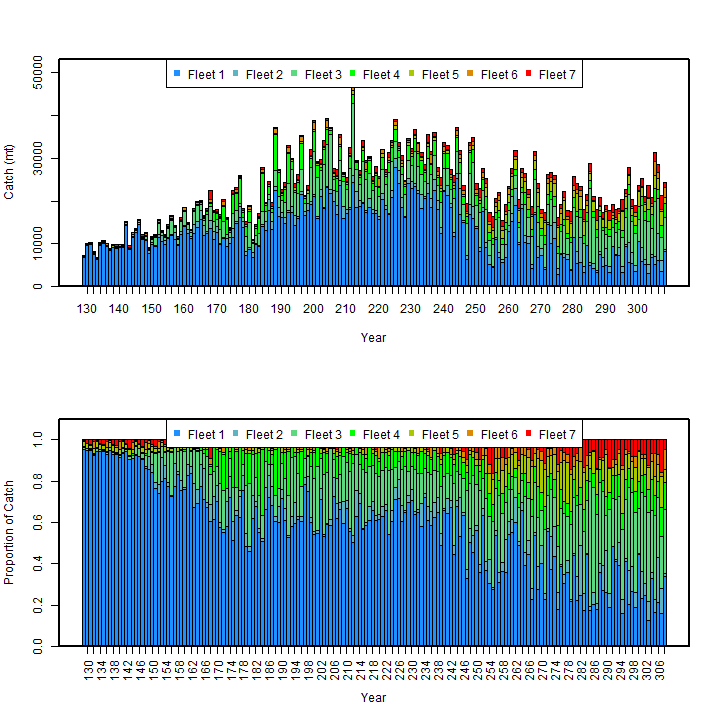
\includegraphics[keepaspectratio]{../figures/fit2/plots_png/input_data/catch_by_fleet.png}}

}

\caption{\label{fig-catch}Absolute and relative annual catch (mt) per
fleet.}

\end{figure}%

\begin{figure}[H]

\centering{

\pandocbounded{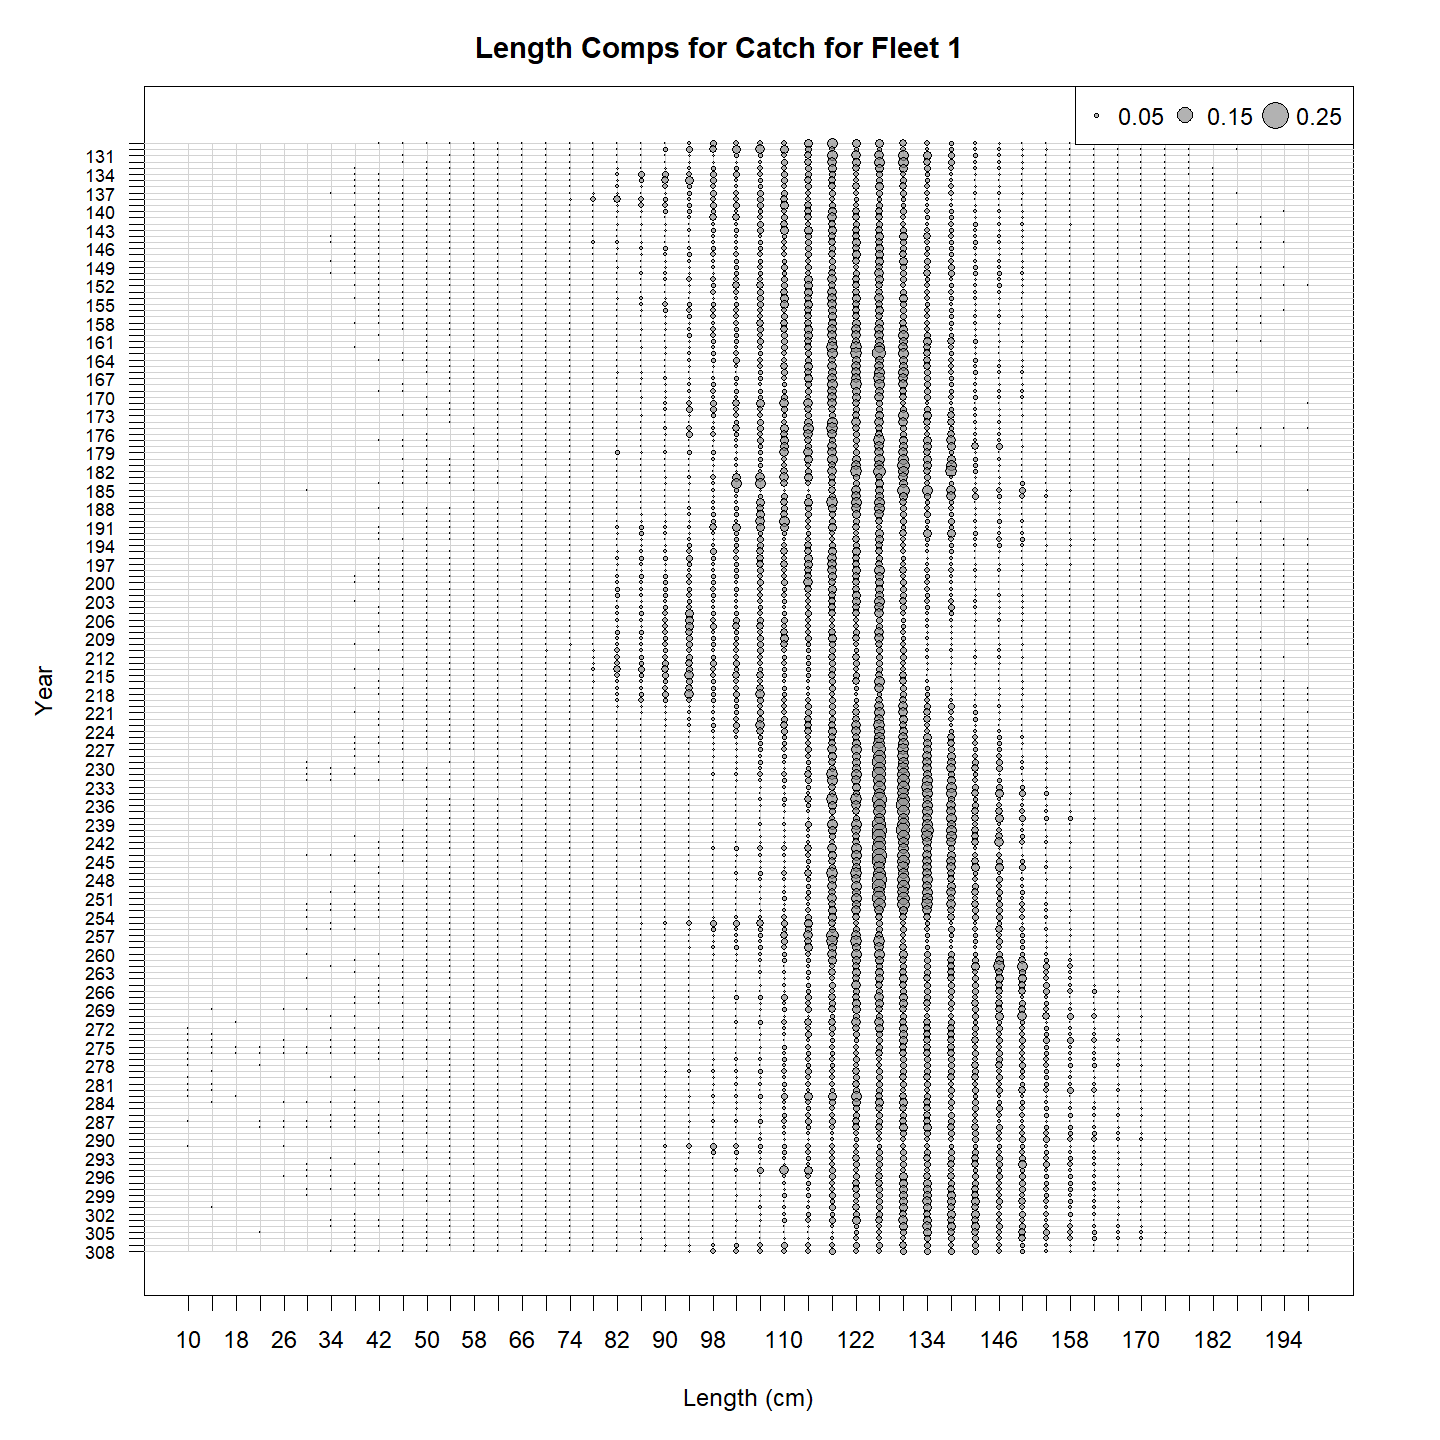
\includegraphics[keepaspectratio]{../figures/fit2/plots_png/input_data/catch_len_comp_fleet_1.png}}

}

\caption{\label{fig-len-1}Yearly marginal length compositions for fleet
LL. Years with gray bubbles were used in the model, while years with
white bubbles were excluded.}

\end{figure}%

\begin{figure}[H]

\centering{

\pandocbounded{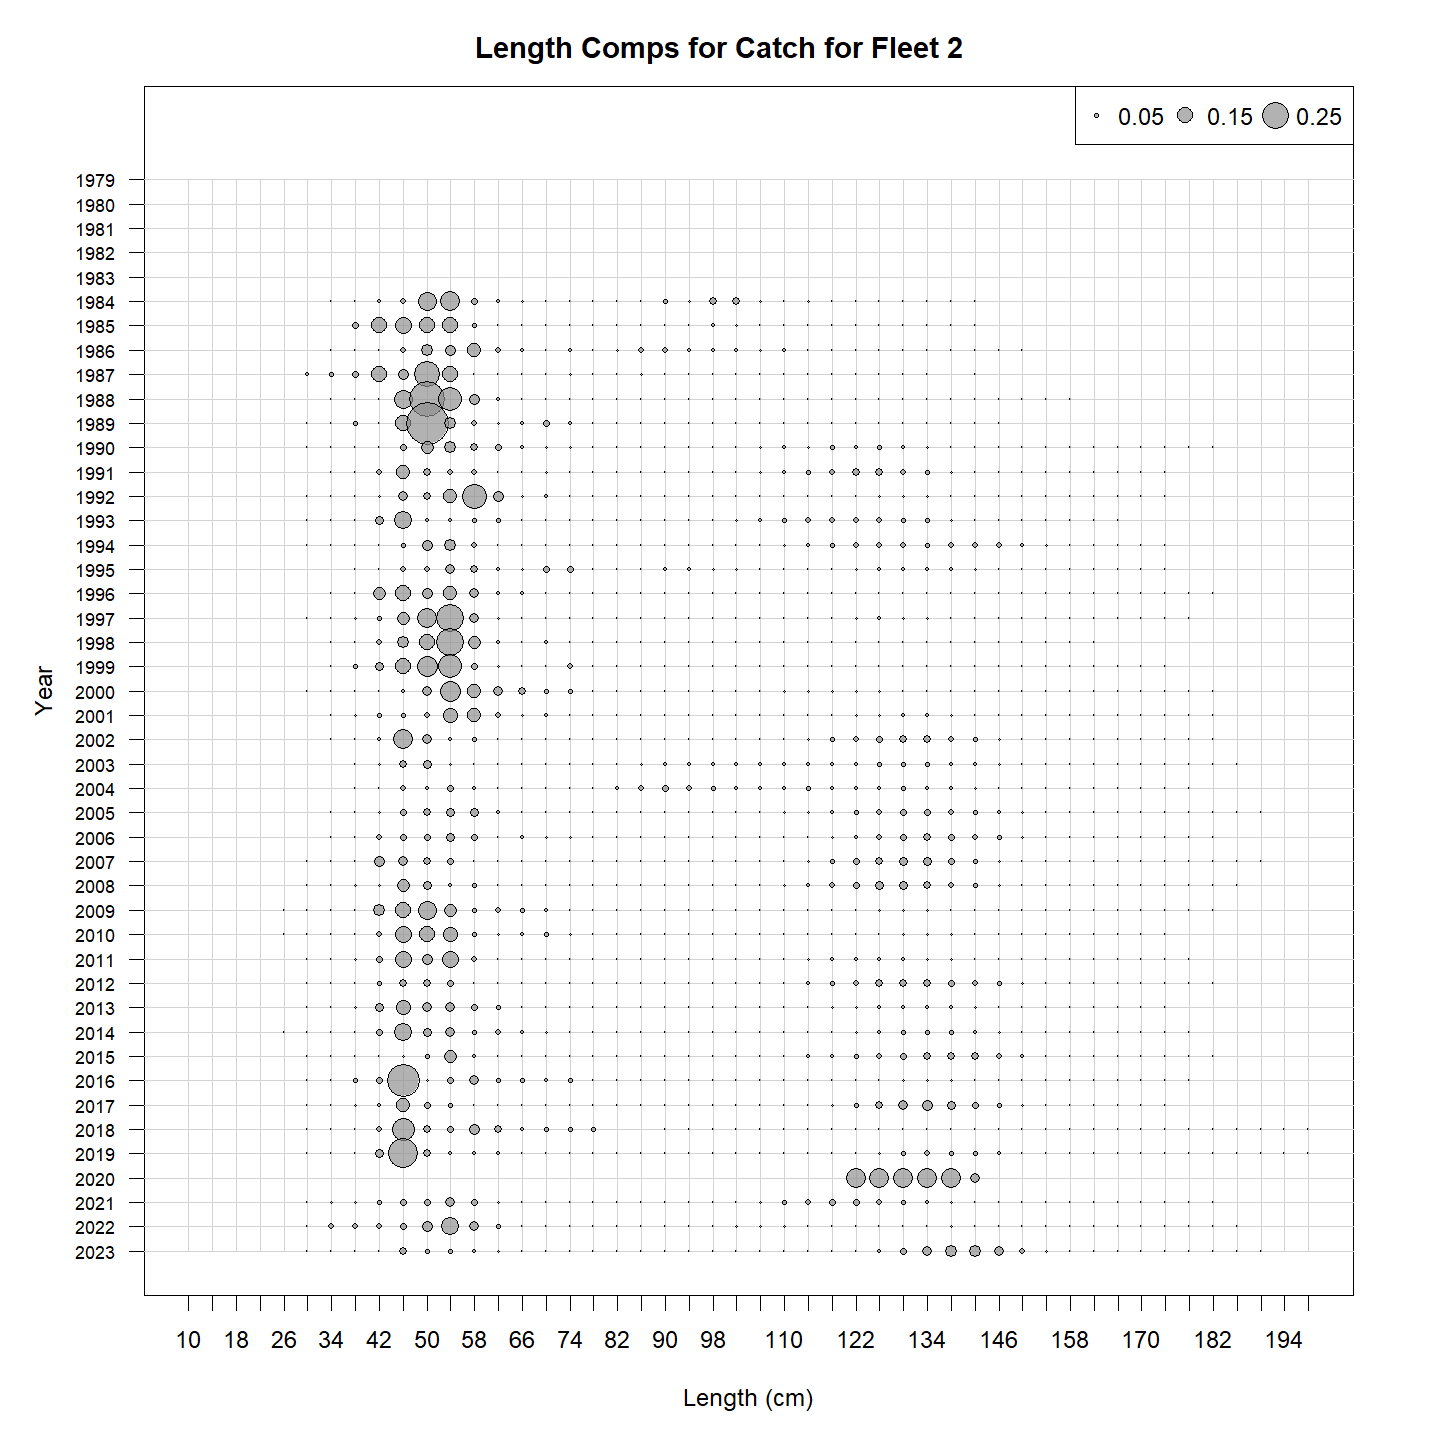
\includegraphics[keepaspectratio]{../figures/fit2/plots_png/input_data/catch_len_comp_fleet_2.png}}

}

\caption{\label{fig-len-2}Yearly marginal length compositions for fleet
PSFS. Years with gray bubbles were used in the model, while years with
white bubbles were excluded.}

\end{figure}%

\begin{figure}[H]

\centering{

\pandocbounded{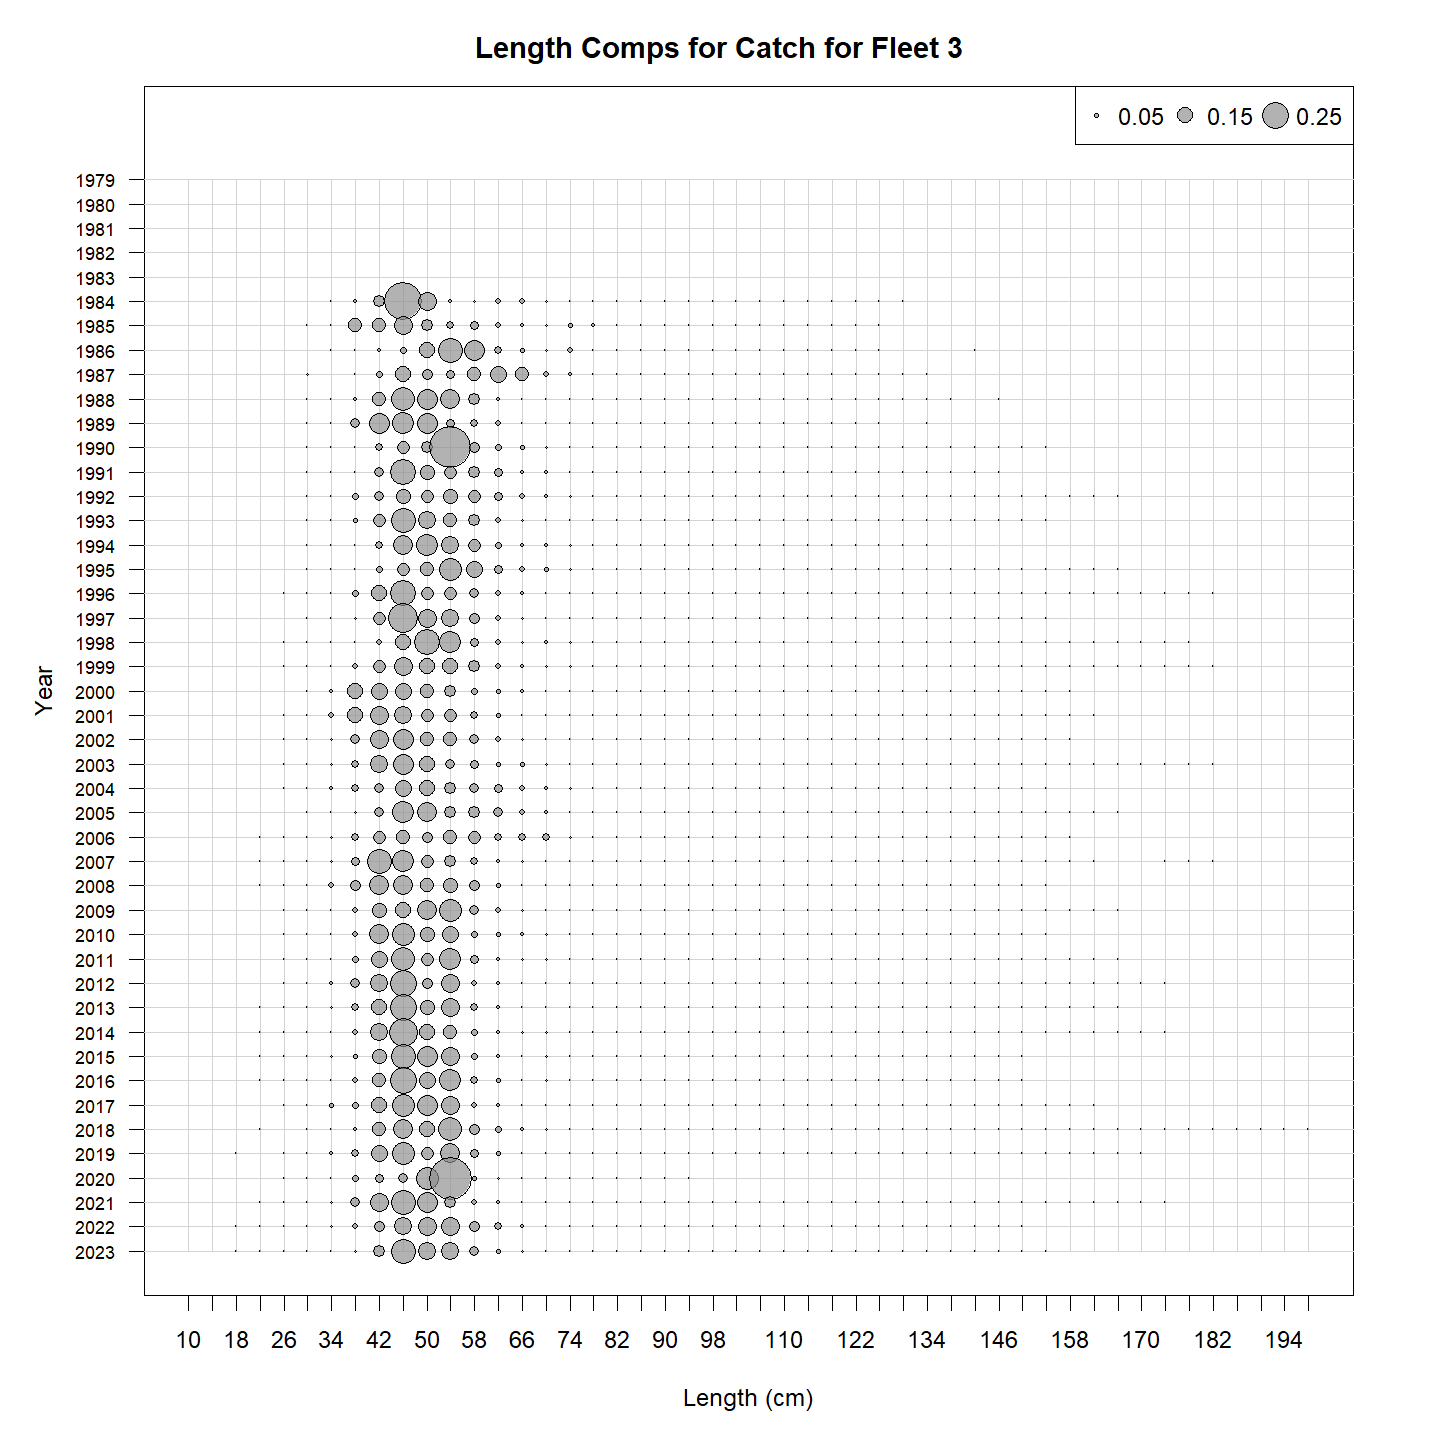
\includegraphics[keepaspectratio]{../figures/fit2/plots_png/input_data/catch_len_comp_fleet_3.png}}

}

\caption{\label{fig-len-3}Yearly marginal length compositions for fleet
PSLS. Years with gray bubbles were used in the model, while years with
white bubbles were excluded.}

\end{figure}%

\begin{figure}[H]

\centering{

\pandocbounded{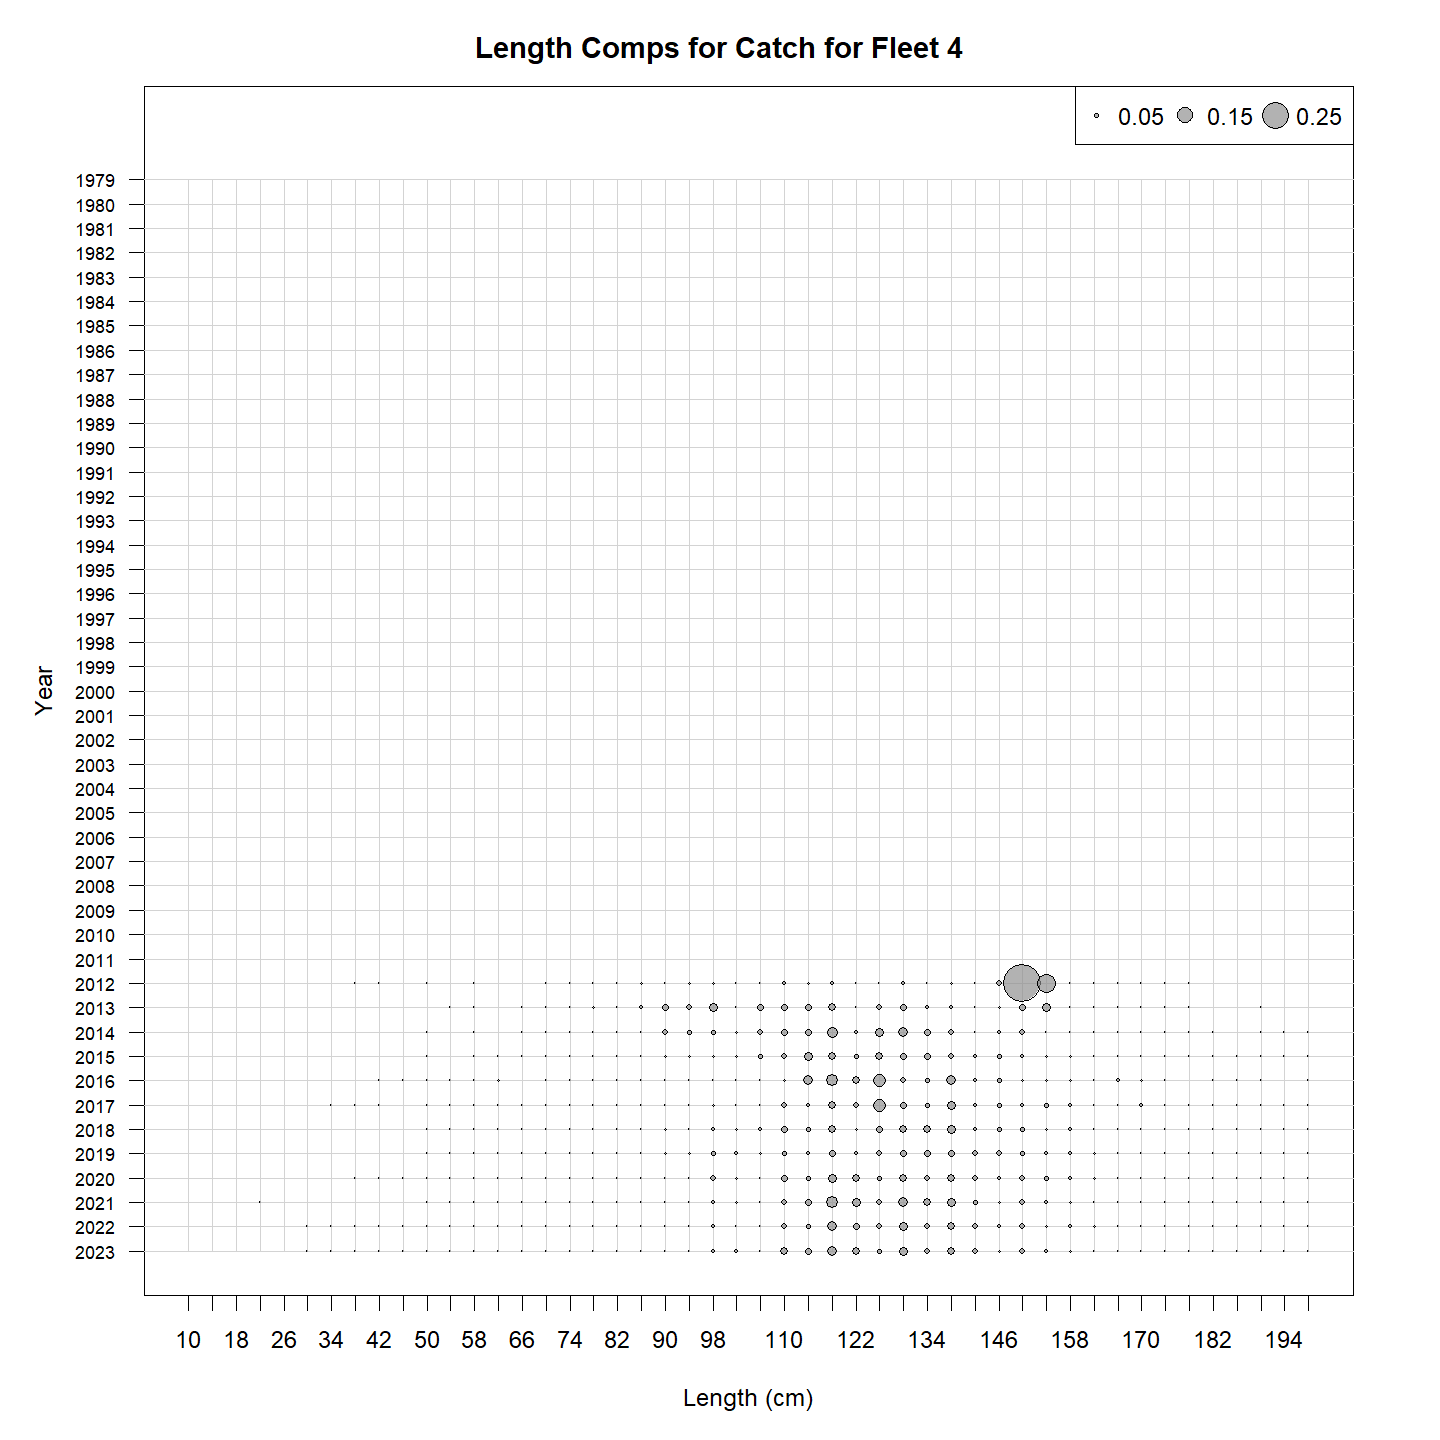
\includegraphics[keepaspectratio]{../figures/fit2/plots_png/input_data/catch_len_comp_fleet_4.png}}

}

\caption{\label{fig-len-4}Yearly marginal length compositions for fleet
FL. Years with gray bubbles were used in the model, while years with
white bubbles were excluded.}

\end{figure}%

\begin{figure}[H]

\centering{

\pandocbounded{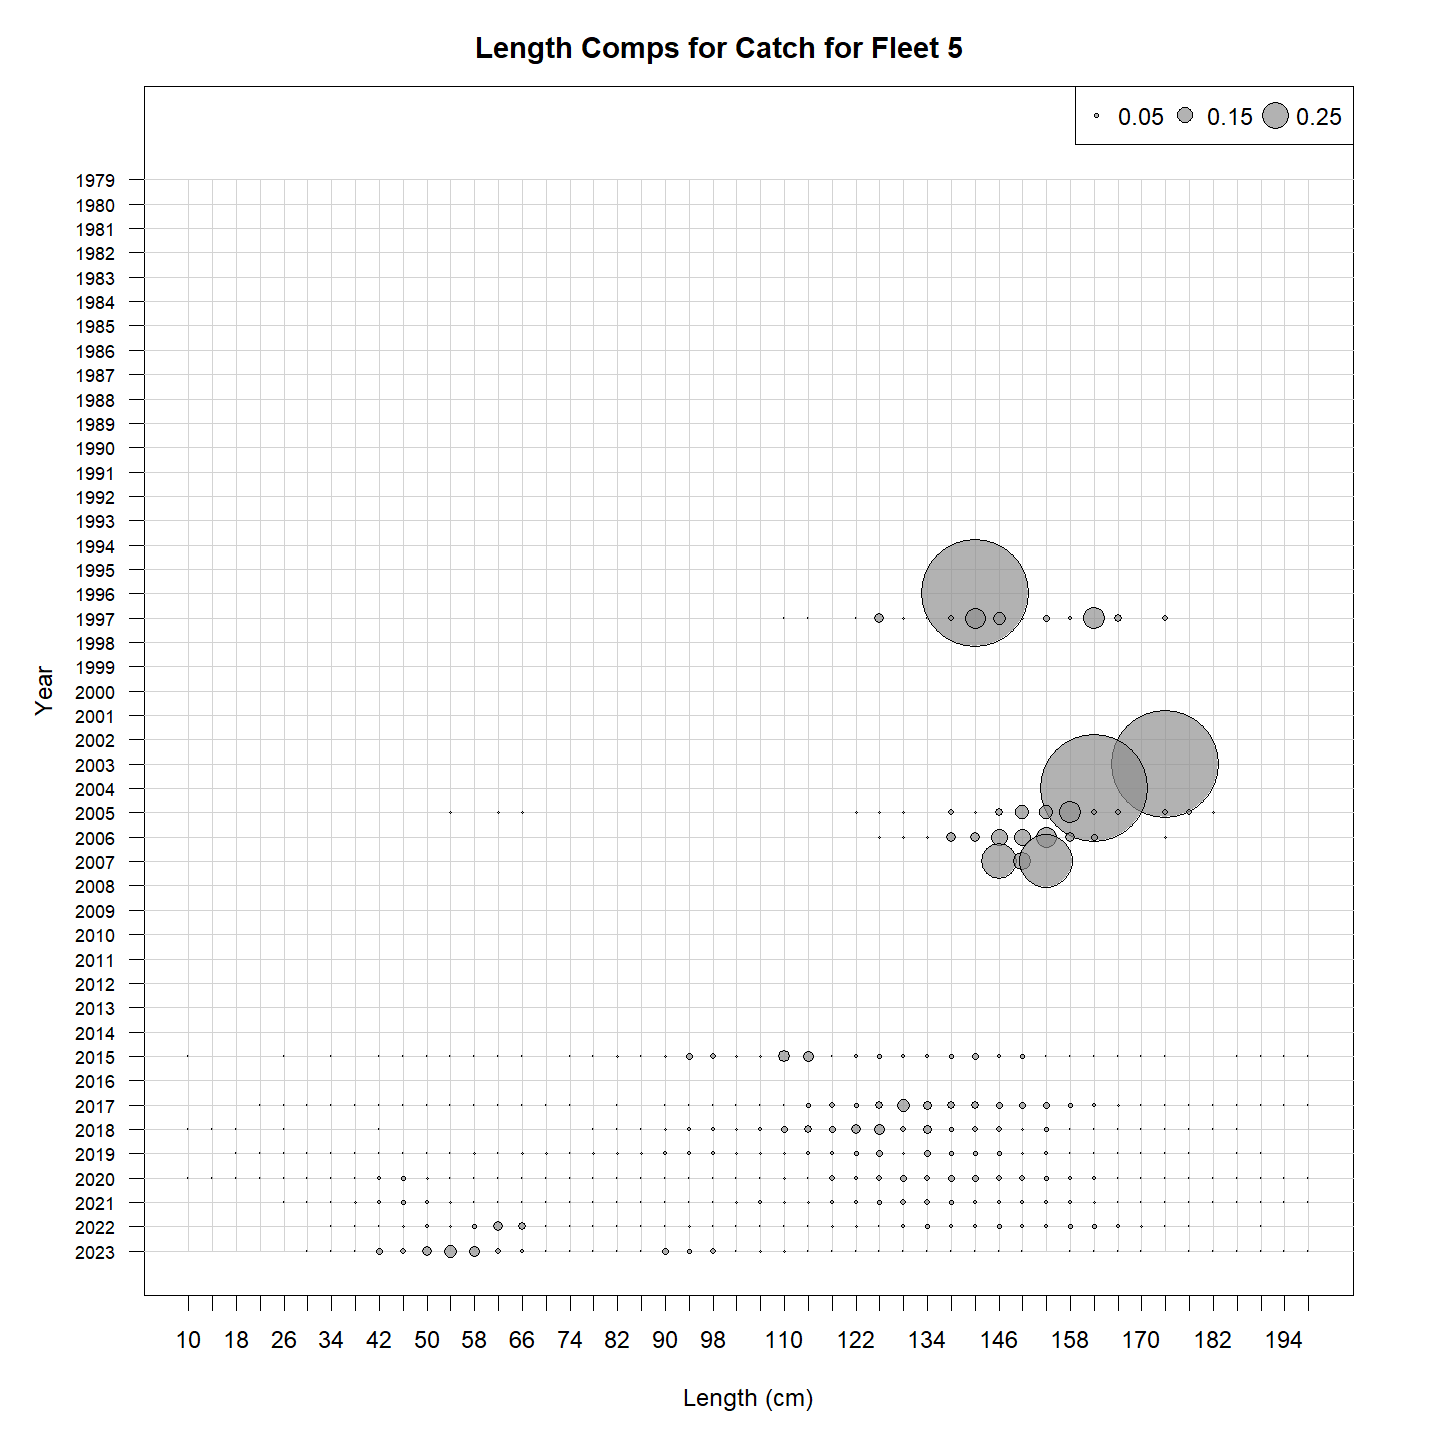
\includegraphics[keepaspectratio]{../figures/fit2/plots_png/input_data/catch_len_comp_fleet_5.png}}

}

\caption{\label{fig-len-5}Yearly marginal length compositions for fleet
LINE. Years with gray bubbles were used in the model, while years with
white bubbles were excluded.}

\end{figure}%

\begin{figure}[H]

\centering{

\pandocbounded{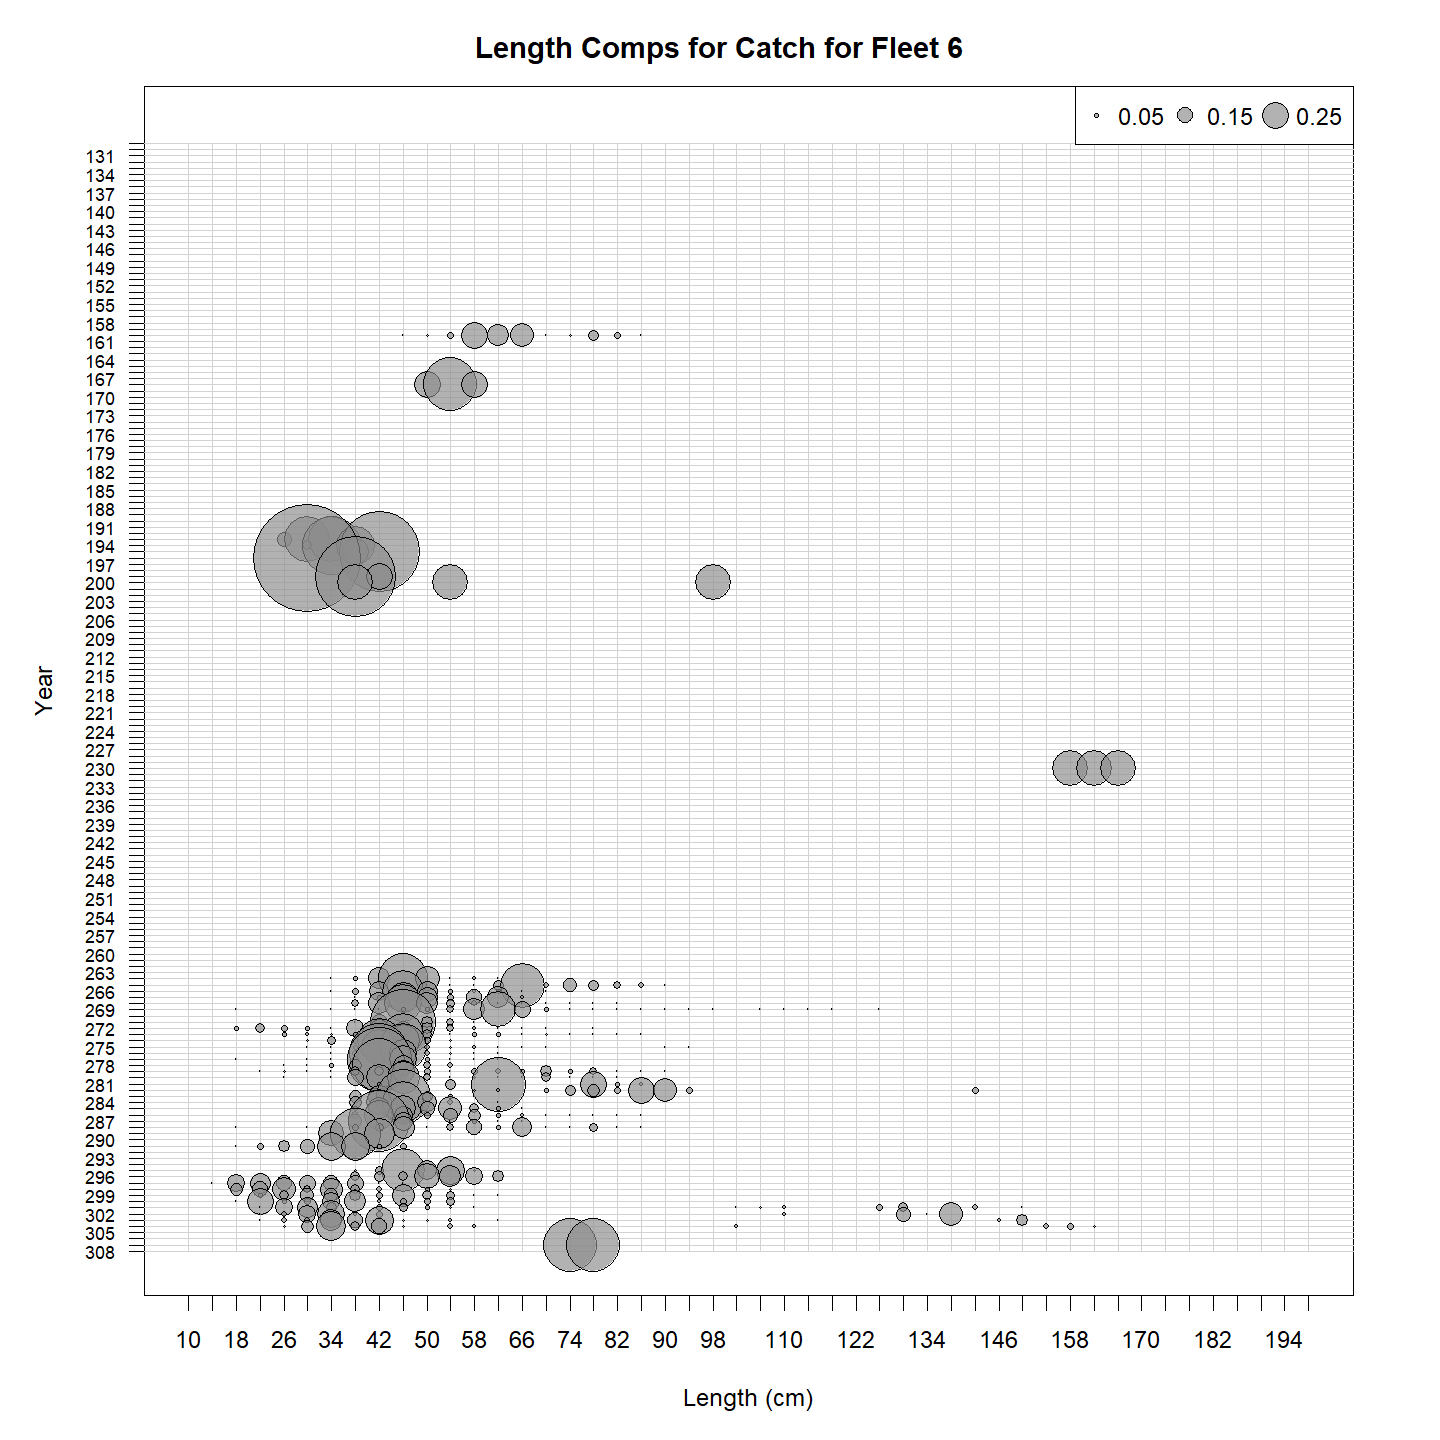
\includegraphics[keepaspectratio]{../figures/fit2/plots_png/input_data/catch_len_comp_fleet_6.png}}

}

\caption{\label{fig-len-6}Yearly marginal length compositions for fleet
BB. Years with gray bubbles were used in the model, while years with
white bubbles were excluded.}

\end{figure}%

\begin{figure}[H]

\centering{

\pandocbounded{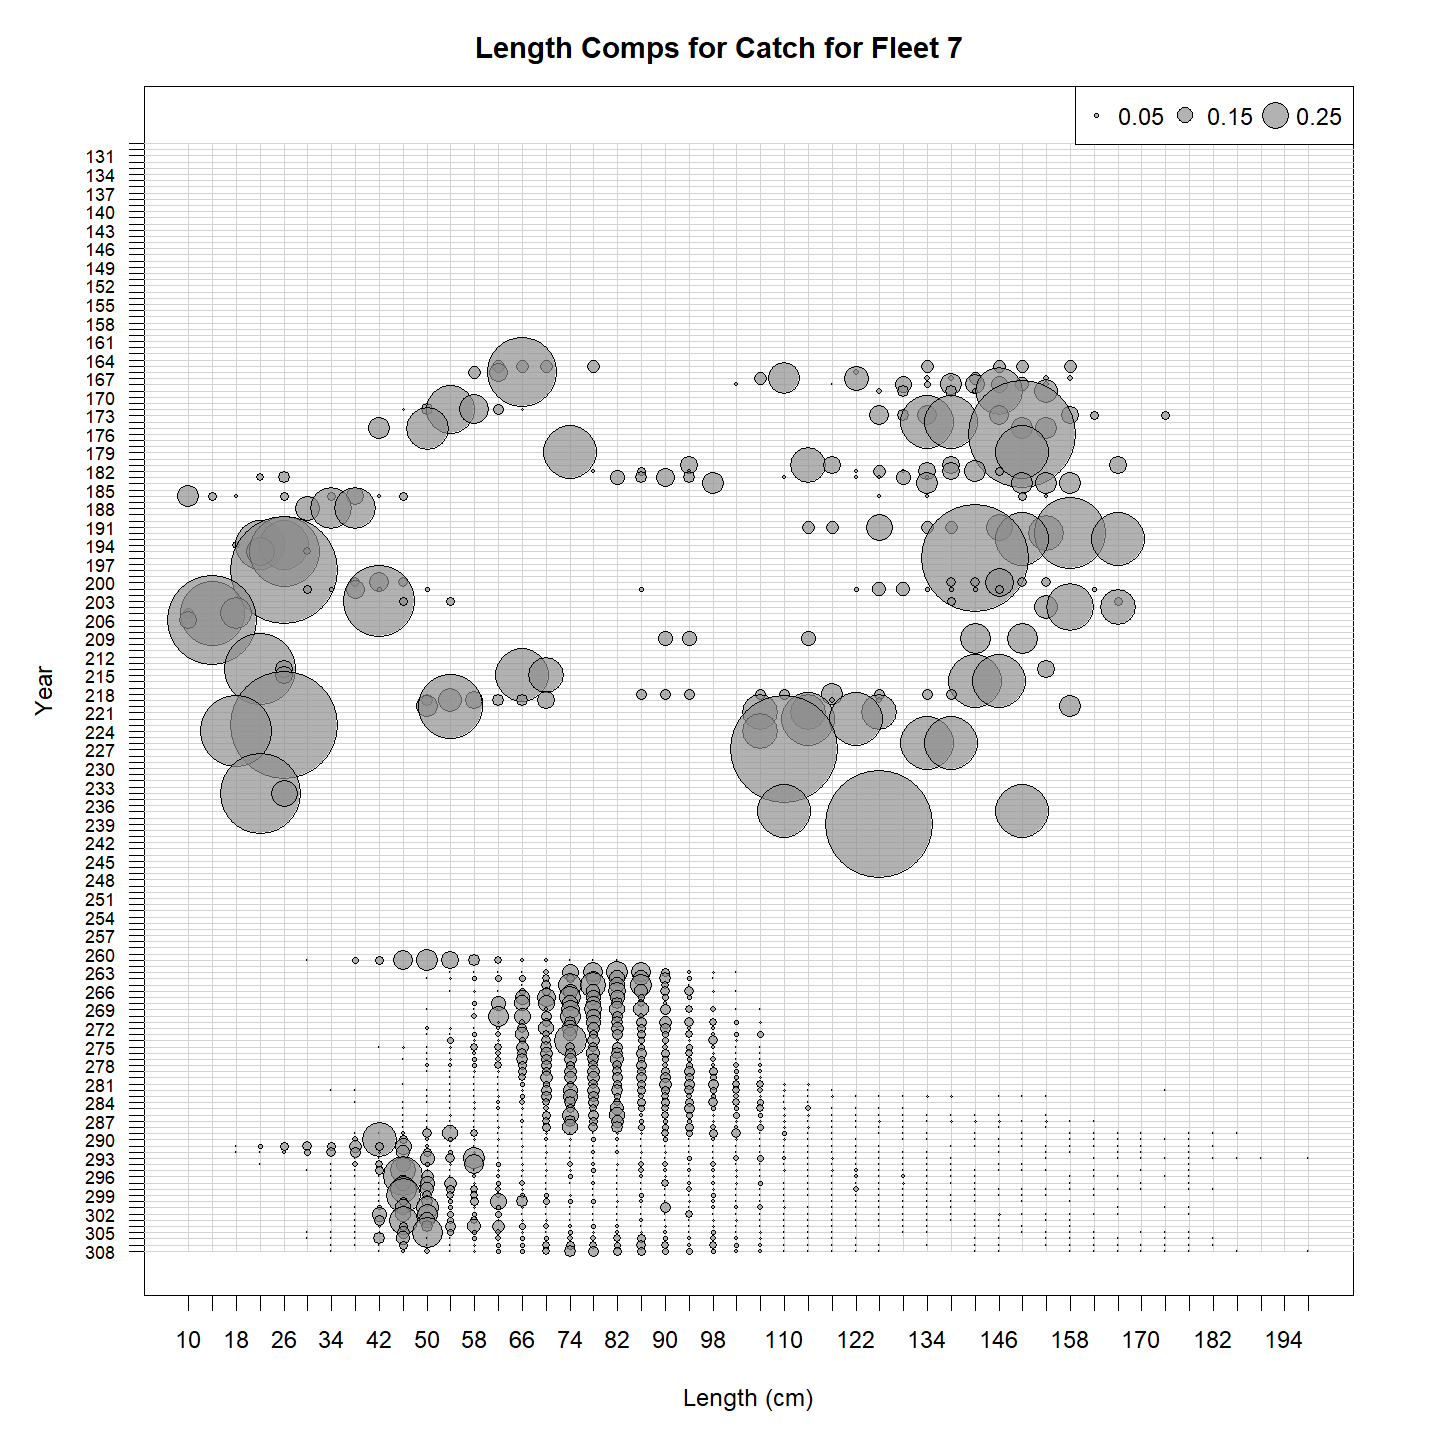
\includegraphics[keepaspectratio]{../figures/fit2/plots_png/input_data/catch_len_comp_fleet_7.png}}

}

\caption{\label{fig-len-7}Yearly marginal length compositions for fleet
OTHER. Years with gray bubbles were used in the model, while years with
white bubbles were excluded.}

\end{figure}%

\begin{figure}[H]

\centering{

\pandocbounded{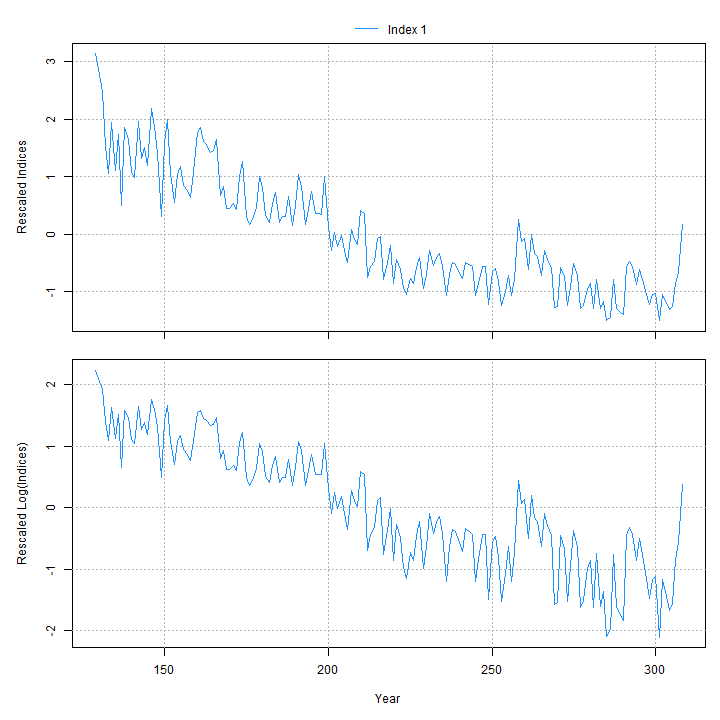
\includegraphics[keepaspectratio]{../figures/fit2/plots_png/input_data/index.png}}

}

\caption{\label{fig-index}Absolute and relative annual catch (mt) per
fleet.}

\end{figure}%

\begin{figure}[H]

\centering{

\pandocbounded{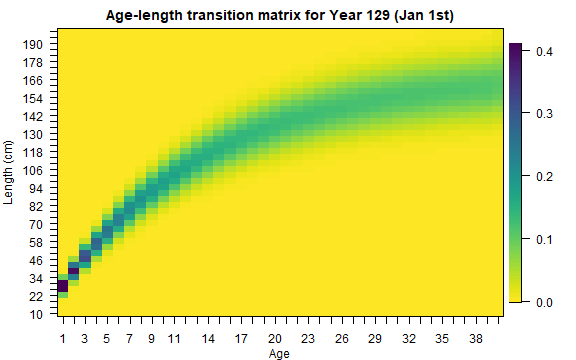
\includegraphics[keepaspectratio]{../figures/fit2/plots_png/results/phi_mat_tile.png}}

}

\caption{\label{fig-growth}Age-length transition matrix. The color scale
indicates the proportion-at-length for each age.}

\end{figure}%

\begin{figure}[H]

\centering{

\pandocbounded{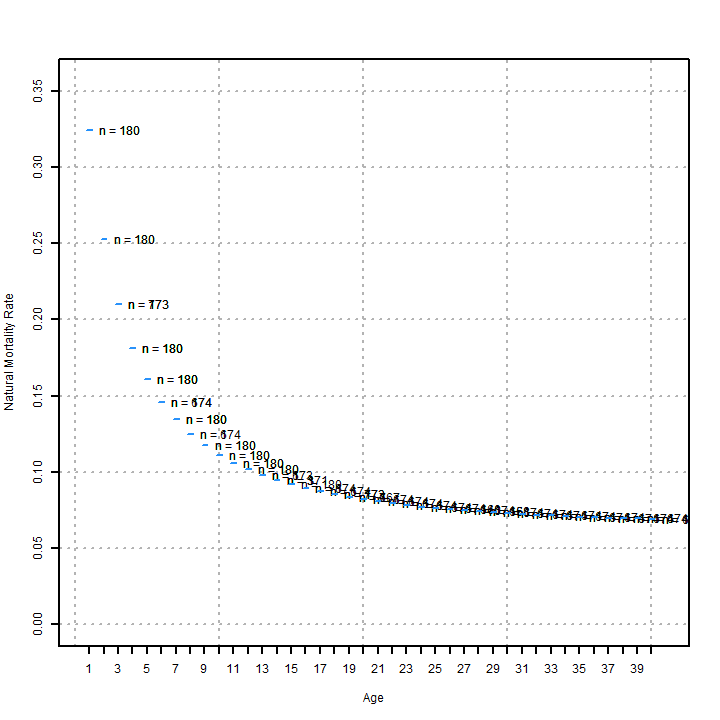
\includegraphics[keepaspectratio]{../figures/fit2/plots_png/results/M_at_age.png}}

}

\caption{\label{fig-Matage}Natural mortality at age derived from the
Lorenzen curve.}

\end{figure}%

\begin{figure}[H]

\centering{

\pandocbounded{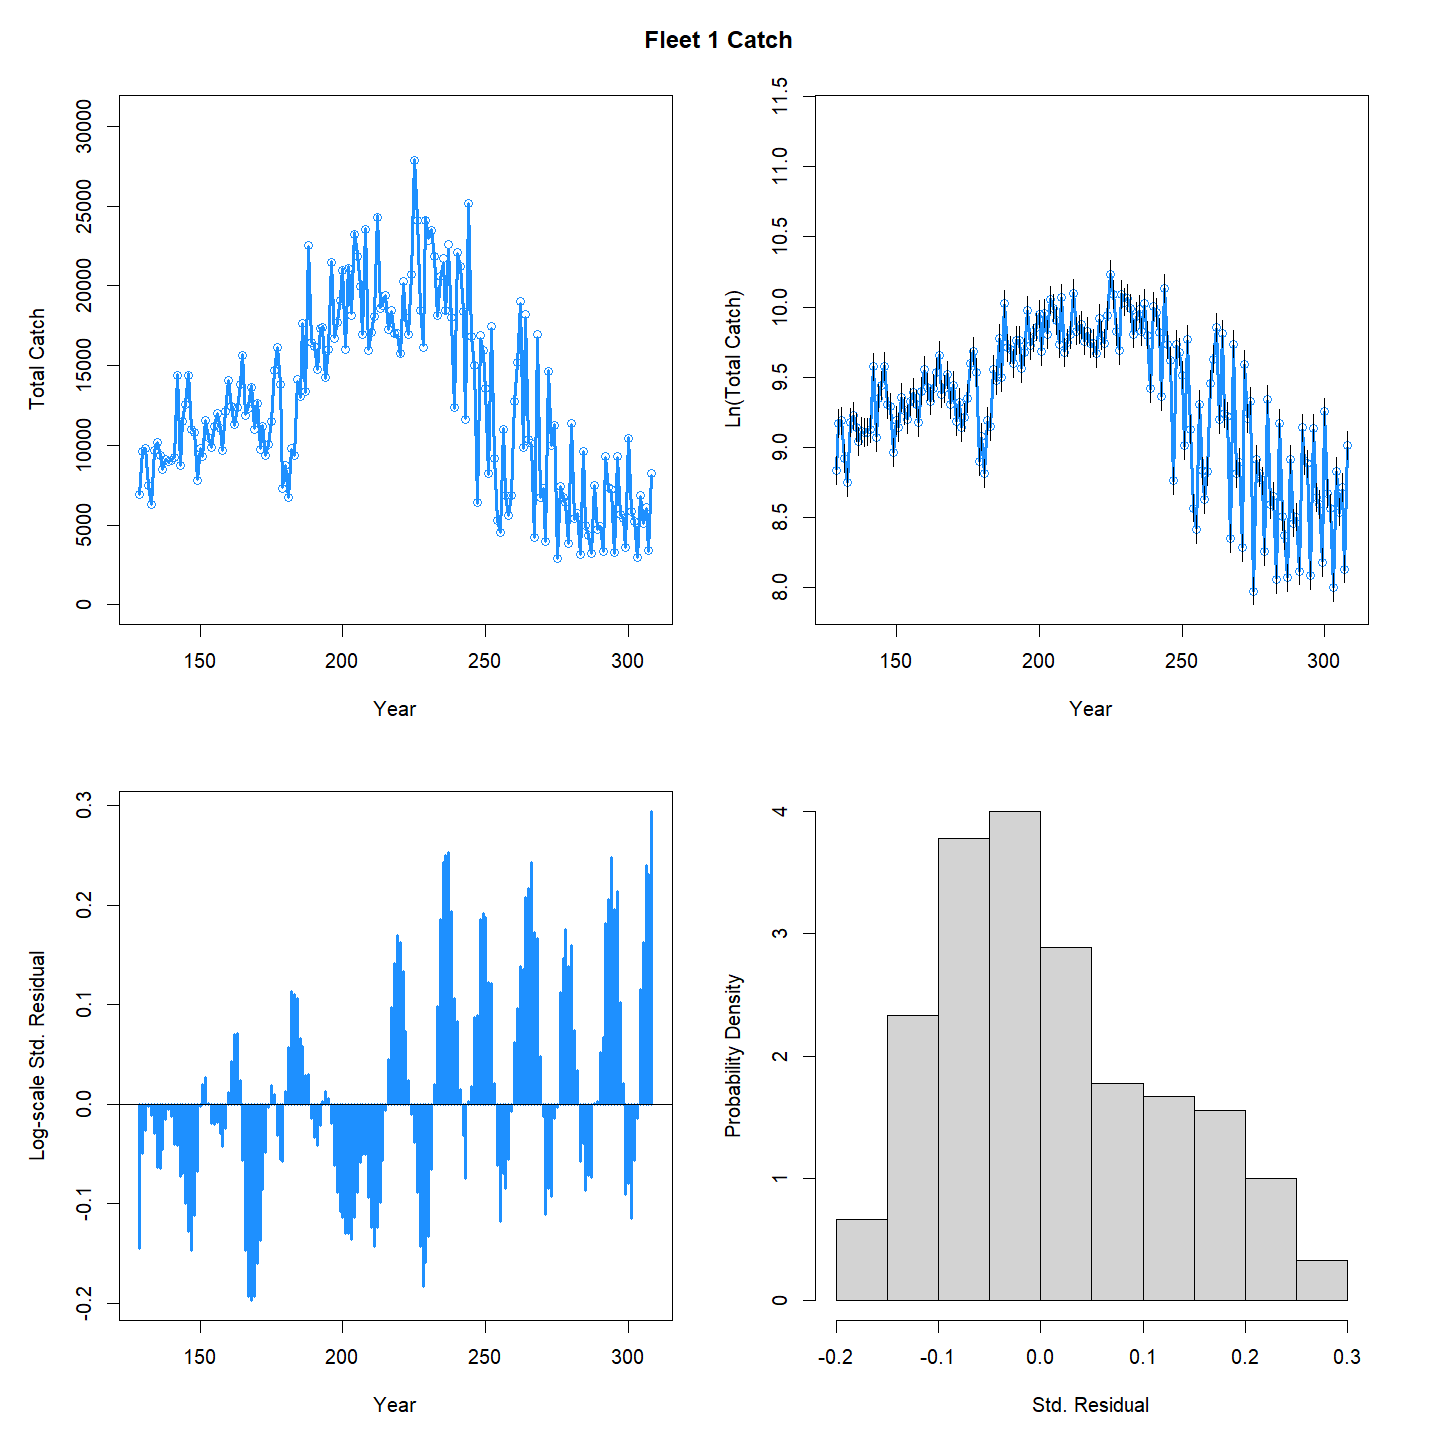
\includegraphics[keepaspectratio]{../figures/fit2/plots_png/diagnostics/Catch_4panel_fleet_1.png}}

}

\caption{\label{fig-fit-catch-ll}Fit to the LL catch data of the
\emph{1BlockLL\_LS\_h08} model configuration. Residuals are also shown
in bottom panels.}

\end{figure}%

\begin{figure}[H]

\centering{

\pandocbounded{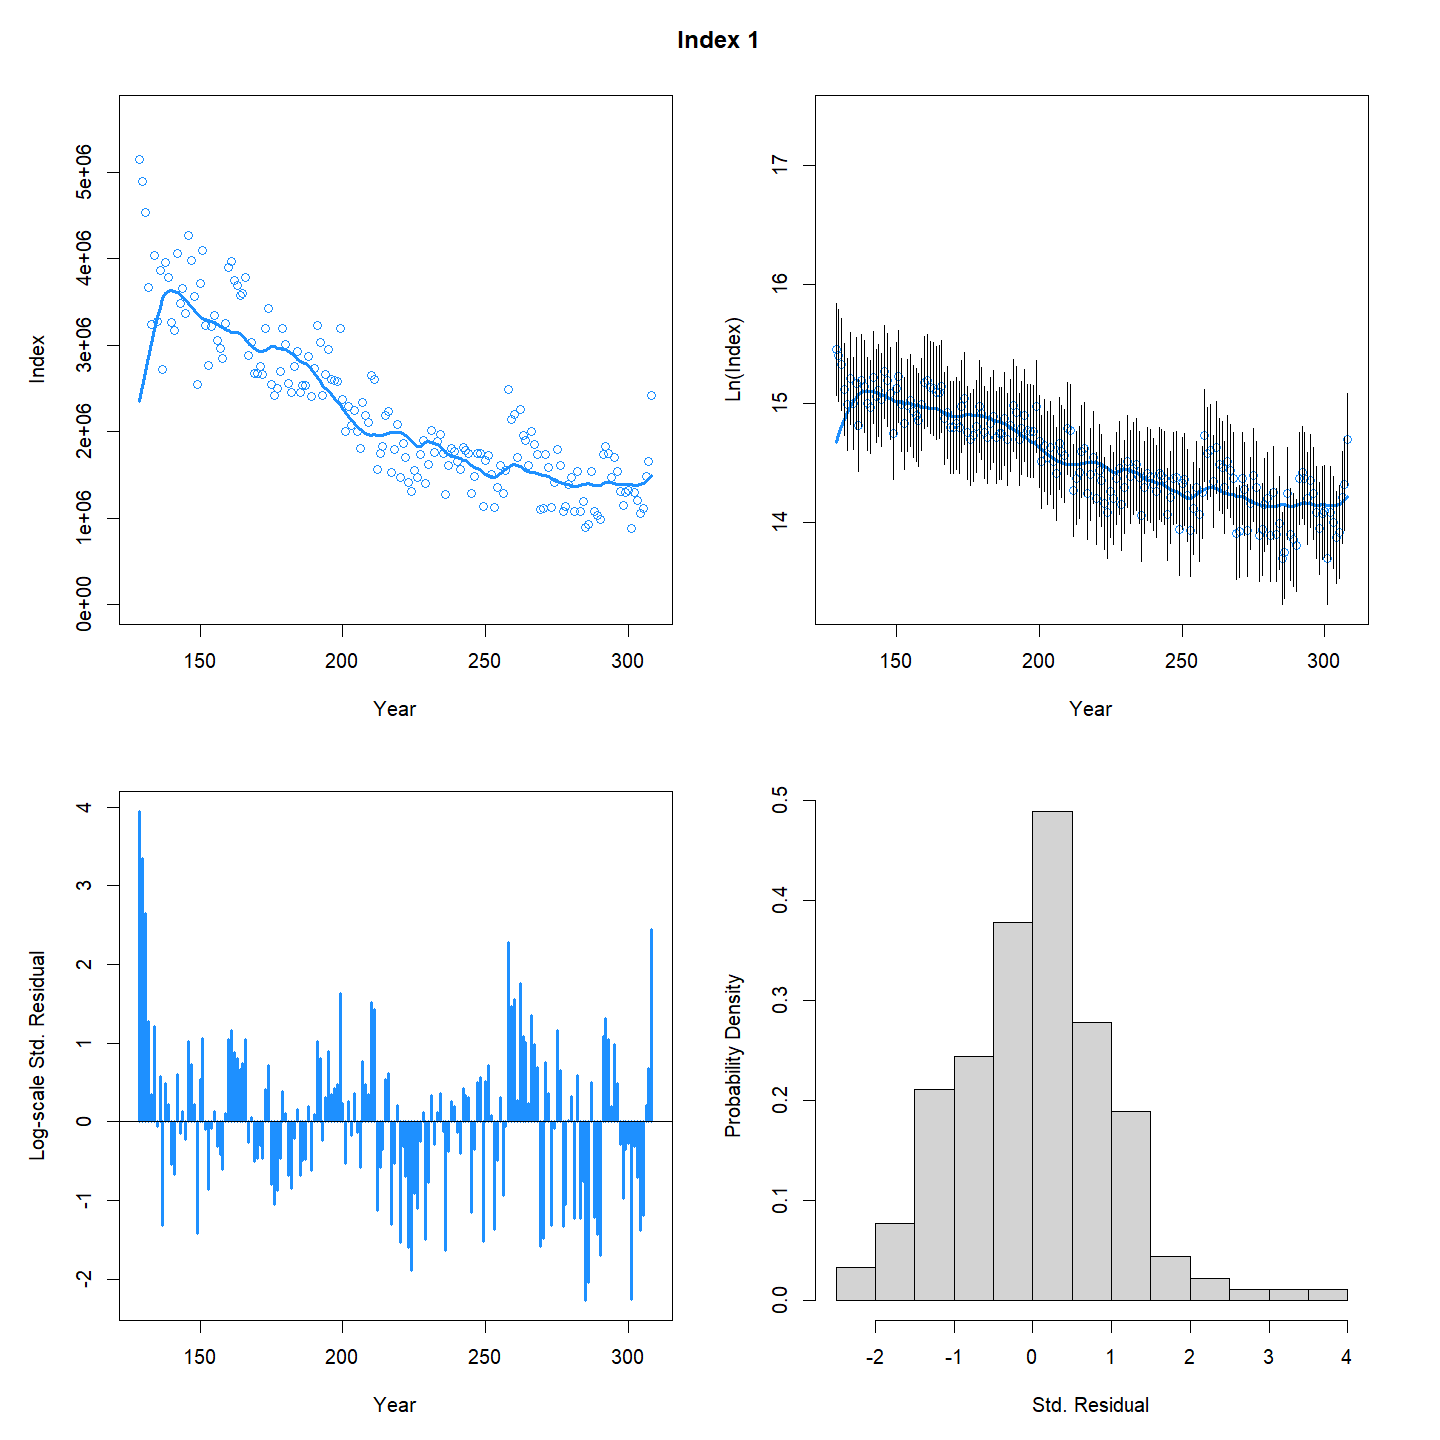
\includegraphics[keepaspectratio]{../figures/fit2/plots_png/diagnostics/Index_4panel_1.png}}

}

\caption{\label{fig-fit-index-ll}Fit to the LL index of the
\emph{1BlockLL\_LS\_h08} model configuration. Residuals are also shown
in bottom panels.}

\end{figure}%

\begin{figure}[H]

\centering{

\pandocbounded{\includegraphics[keepaspectratio]{../figures/fit2/plots_png/diagnostics/Index_4panel_2.png}}

}

\caption{\label{fig-fit-index-ls}Fit to the PSLS index of the
\emph{1BlockLL\_LS\_h08}. Residuals are also shown in bottom panels.}

\end{figure}%

\begin{figure}[H]

\centering{

\pandocbounded{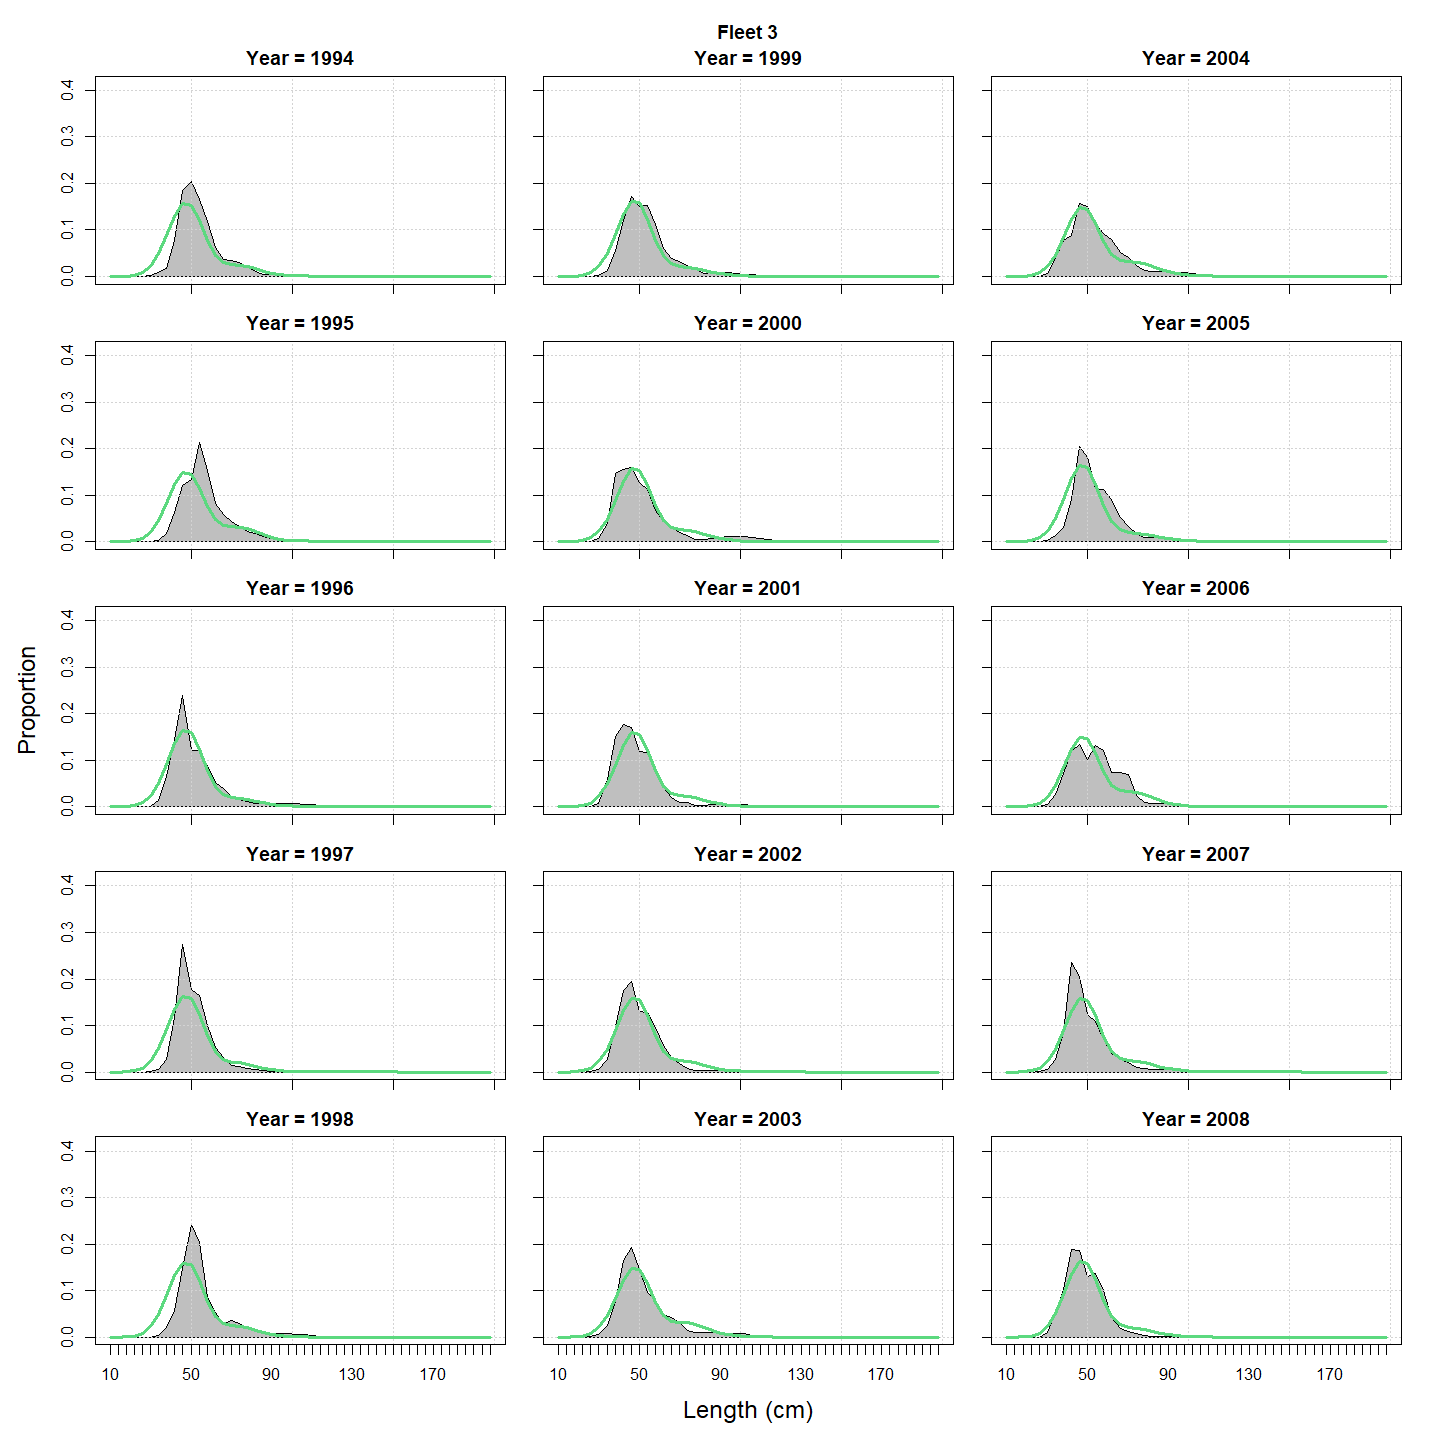
\includegraphics[keepaspectratio]{../figures/fit2/plots_png/diagnostics/Catch_len_comp_fleet_3_a.png}}

}

\caption{\label{fig-fit-len-ls}Example of annual fits to PSLS length
compositions of the \emph{1BlockLL\_LS\_h08} model configuration.}

\end{figure}%

\begin{figure}[H]

\centering{

\pandocbounded{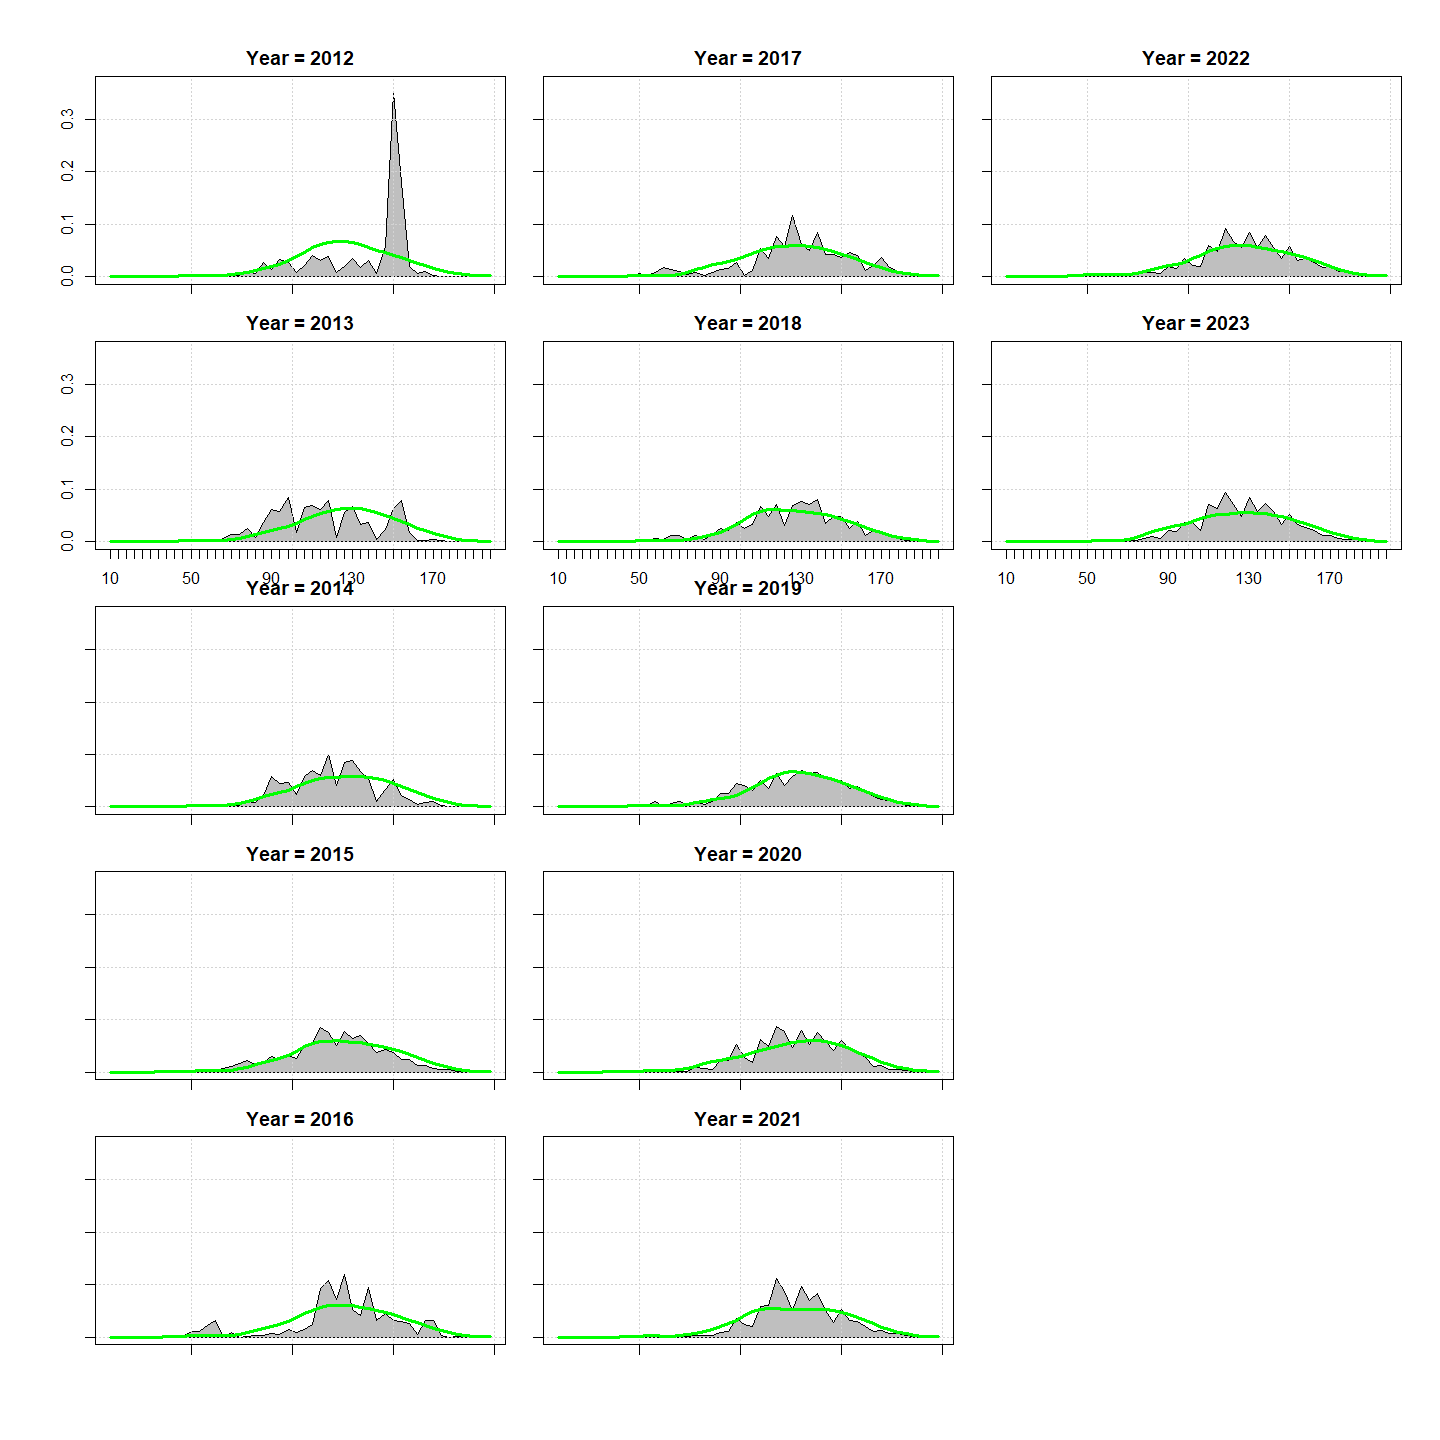
\includegraphics[keepaspectratio]{../figures/fit2/plots_png/diagnostics/Catch_len_comp_fleet_4.png}}

}

\caption{\label{fig-fit-len-fl}Example of annual fits to FL length
compositions of the \emph{1BlockLL\_LS\_h08} model configuration.}

\end{figure}%

\begin{figure}[H]

\centering{

\pandocbounded{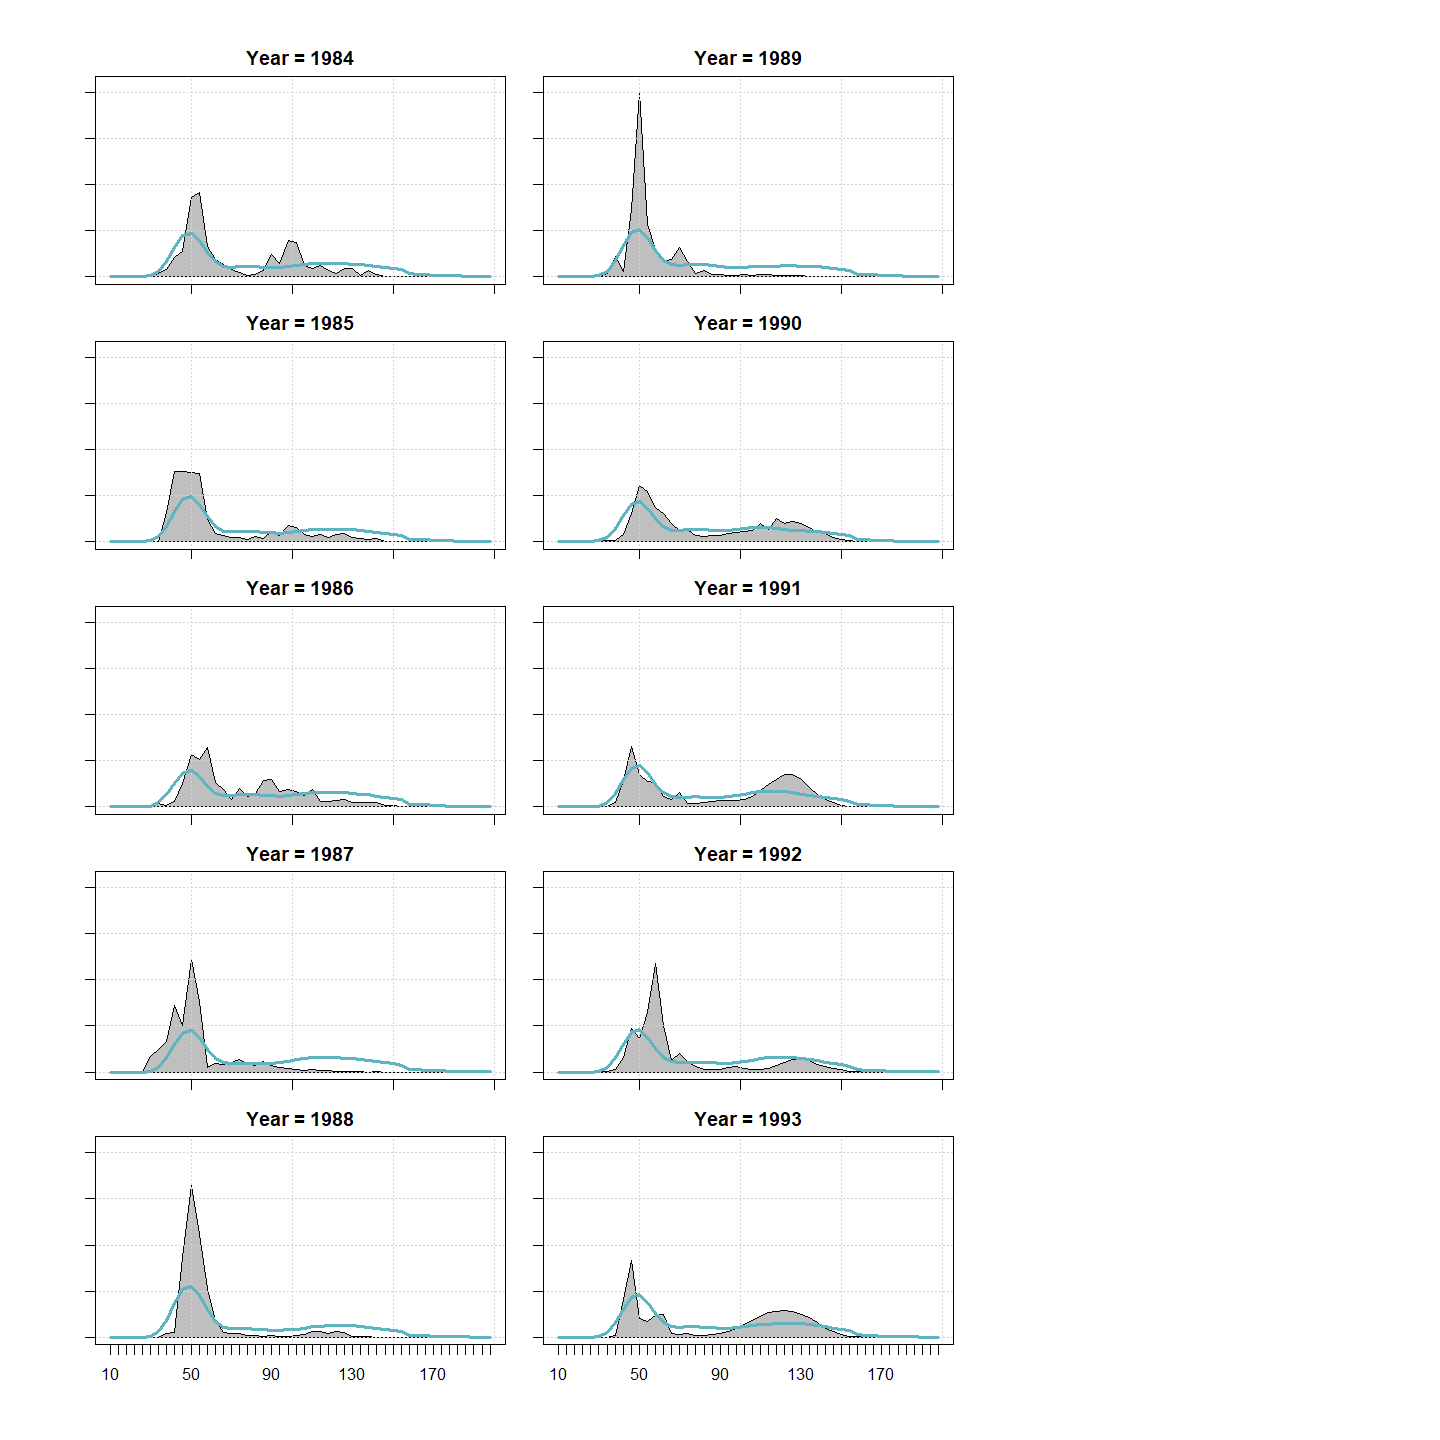
\includegraphics[keepaspectratio]{../figures/fit2/plots_png/diagnostics/Catch_len_comp_fleet_2.png}}

}

\caption{\label{fig-fit-len-fs}Example of annual fits to PSFS length
compositions of the \emph{1BlockLL\_LS\_h08} model configuration.}

\end{figure}%

\begin{figure}[H]

\centering{

\pandocbounded{\includegraphics[keepaspectratio]{../figures/fit2/plots_png/diagnostics/Catch_len_comp_fleet_1.png}}

}

\caption{\label{fig-fit-len-ll-1}Example of annual fits to LL length
compositions of the \emph{1BlockLL\_LS\_h08} model configuration.}

\end{figure}%

\begin{figure}[H]

\centering{

\pandocbounded{\includegraphics[keepaspectratio]{../figures/fit4/plots_png/diagnostics/Catch_len_comp_fleet_1.png}}

}

\caption{\label{fig-fit-len-ll-2}Example of annual fits to LL length
compositions of the \emph{2BlockLL\_LS\_h08} model configuration.}

\end{figure}%

\begin{figure}[H]

\centering{

\pandocbounded{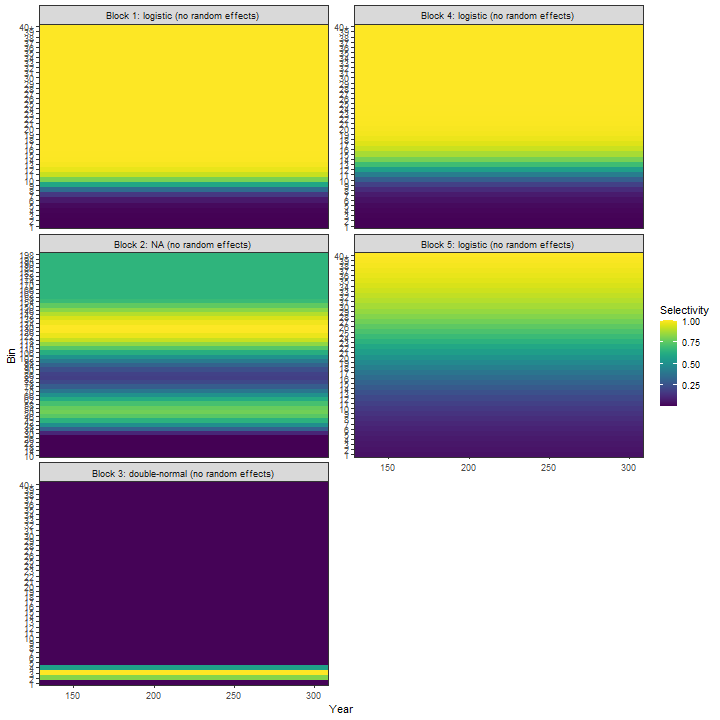
\includegraphics[keepaspectratio]{../figures/fit2/plots_png/results/selex_tile.png}}

}

\caption{\label{fig-res-selex-1}Selectivity per fleet estimated by the
\emph{1BlockLL\_LS\_h08} model configuration.}

\end{figure}%

\begin{figure}[H]

\centering{

\pandocbounded{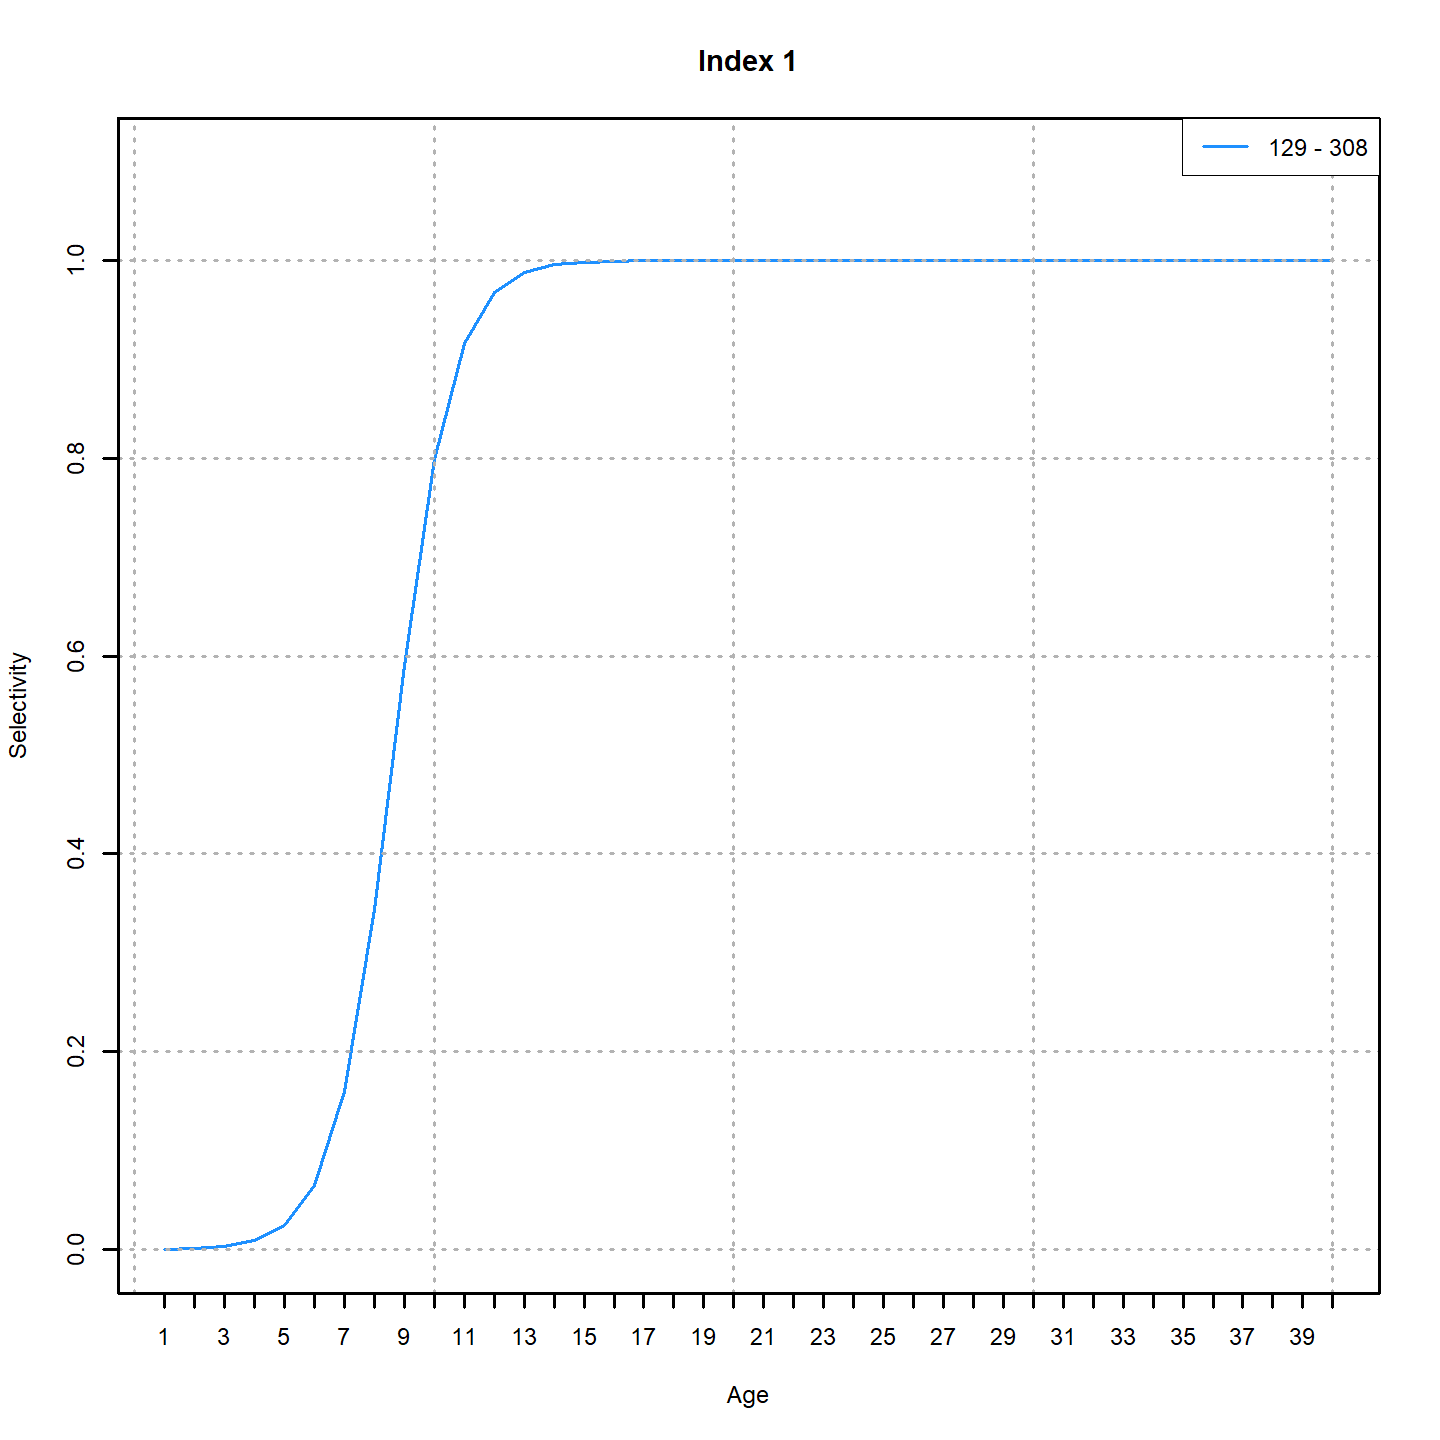
\includegraphics[keepaspectratio]{../figures/fit4/plots_png/results/Selectivity_index1.png}}

}

\caption{\label{fig-res-selex-2}Selectivity for the LL fleet estimated
by the \emph{2BlockLL\_LS\_h08} model configuration.}

\end{figure}%

\begin{figure}[H]

\centering{

\pandocbounded{\includegraphics[keepaspectratio]{../figures/fit2/plots_png/results/SSB_Rec.png}}

}

\caption{\label{fig-res-ssr}Relationship between annual estimates of SSB
and recruitment by the \emph{1BlockLL\_LS\_h08} model configuration.}

\end{figure}%

\begin{figure}[H]

\centering{

\pandocbounded{\includegraphics[keepaspectratio]{../figures/compare/compare_png/compare_SSB_F_R.png}}

}

\caption{\label{fig-comp-ts}Comparison of annual estimates of SSB,
recruitment, and fishing mortality among the model configurations.}

\end{figure}%

\begin{figure}[H]

\centering{

\pandocbounded{\includegraphics[keepaspectratio]{../figures/compare/compare_png/compare_ref_pts.png}}

}

\caption{\label{fig-comp-ref-1}Annual estimates of \(SSB_{MSY}\),
\(MSY\), and \(F_{MSY}\) by the model configurations.}

\end{figure}%

\begin{figure}[H]

\centering{

\pandocbounded{\includegraphics[keepaspectratio]{../figures/compare/compare_png/compare_rel_status_timeseries.png}}

}

\caption{\label{fig-comp-ref-2}Annual estimates of \(SSB/SSB_{MSY}\) and
\(F/F_{MSY}\) by the model configurations.}

\end{figure}%

\begin{figure}[H]

\centering{

\pandocbounded{\includegraphics[keepaspectratio]{../figures/compare/compare_png/compare_rel_status_kobe.png}}

}

\caption{\label{fig-kobe}Stock status (Kobe plot) estimated by the model
configurations.}

\end{figure}%

\begin{figure}[H]

\centering{

\pandocbounded{\includegraphics[keepaspectratio]{../figures/fit3/plots_png/retro/SSB_retro.png}}

}

\caption{\label{fig-retro-ssb}Retrospective patterns in SSB by the
\emph{2BlockLL\_noLS} model.}

\end{figure}%

\begin{figure}[H]

\centering{

\pandocbounded{\includegraphics[keepaspectratio]{../figures/fit3/plots_png/retro/SSB_MSY_retro.png}}

}

\caption{\label{fig-retro-ssbmsy}Retrospective patterns in
\(SSB/SSB_{msy}\) by the \emph{2BlockLL\_noLS} model.}

\end{figure}%

\begin{figure}[H]

\centering{

\pandocbounded{\includegraphics[keepaspectratio]{../figures/fit3/plots_png/retro/NAA_age1_retro.png}}

}

\caption{\label{fig-retro-rec}Retrospective patterns in recruitment by
the \emph{2BlockLL\_noLS} model.}

\end{figure}%

\begin{figure}[H]

\centering{

\pandocbounded{\includegraphics[keepaspectratio]{../figures/fit3/plots_png/retro/Fbar_retro.png}}

}

\caption{\label{fig-retro-f}Retrospective patterns in fishing mortality
(averaged for ages 1-5) by the \emph{2BlockLL\_noLS} model.}

\end{figure}%

\begin{figure}[H]

\centering{

\pandocbounded{\includegraphics[keepaspectratio]{../figures/jitter/nLL.png}}

}

\caption{\label{fig-jitter-nll}Jitter analysis by model configuration.
Change in marginal negative log likelihood by jitter iteration (x-axis).
Ten iterations were run.}

\end{figure}%

\begin{figure}[H]

\centering{

\pandocbounded{\includegraphics[keepaspectratio]{../figures/jitter/SSB.png}}

}

\caption{\label{fig-jitter-ssb}Jitter analysis by model configuration.
Change in estimates of annual SSB. Ten iterations were run.}

\end{figure}%

\begin{figure}[H]

\centering{

\pandocbounded{\includegraphics[keepaspectratio]{../figures/profile_N1/nLL.png}}

}

\caption{\label{fig-prof-N1}Likelihood profile of initial abundance at
age 1 (\(N_1\)) for the \emph{1BlockLL\_LS} model configuration. The
profile is shown by likelihood component. The dashed vertical line
represents the parameter value used in the model.}

\end{figure}%

\begin{figure}[H]

\centering{

\pandocbounded{\includegraphics[keepaspectratio]{../figures/proj/SSB.png}}

}

\caption{\label{fig-proj-ssb}Five-year projection in SSB and
\(SSB_{MSY}\) by model configuration. The projected F was assumed to be
as in 2024. The vertical dashed line indicates the start of the
projection.}

\end{figure}%

\begin{figure}[H]

\centering{

\pandocbounded{\includegraphics[keepaspectratio]{../figures/proj/catch.png}}

}

\caption{\label{fig-proj-catch}Five-year projection in total catch and
\(MSY\) by model configuration. The projected F was assumed to be as in
2024. The vertical dashed line indicates the start of the projection.}

\end{figure}%




\end{document}
